\documentclass[12pt, a4paper, notitlepage]{article}

\usepackage[utf8]{inputenc}
\usepackage{amsmath}
\usepackage{mathtools}
\usepackage{amsfonts}
\usepackage[a4paper,left=1.5in,right=1in,top=1in,bottom=1in]{geometry}
\usepackage{setspace}
\usepackage[nottoc, numbib]{tocbibind}
\usepackage{multicol}
\usepackage[font=small]{caption}
\usepackage{graphicx}
\usepackage{float}
\usepackage[hidelinks]{hyperref}
\usepackage{multirow}
\usepackage{censor}
\onehalfspacing

\makeatletter
\renewcommand*\l@figure{\@dottedtocline{1}{1.5em}{2.75em}}
\let\l@table\l@figure
\makeatother

\usepackage{xcolor,colortbl}
\definecolor{Gray}{gray}{0.85}
\definecolor{LightCyan}{rgb}{0.88,1,1}
\definecolor{LightGreen}{RGB}{144,238,144}
\def\code#1{\texttt{#1}}

\numberwithin{equation}{subsection}
\numberwithin{figure}{subsection}
\numberwithin{table}{subsection}
\setlength\parindent{0pt}
\setlength{\fboxsep}{0pt}

\newcommand\numberthis{\addtocounter{equation}{1}\tag{\theequation}}
\newcommand{\img}[3]
{
    \begin{figure}[H]
	\caption{#1}
	\centerline{\fbox{\includegraphics[width=1\textwidth]{#2}}}
	\label{#3}
    \end{figure}
}

\newif\ifhidesecrets
\hidesecretsfalse

\newcommand{\newpar}{\newline \newline}
\newcommand{\lambdaVect}{\pmb{\lambda}}
\newcommand{\mathFor}{ \text{for} \quad}

\renewcommand{\abstractname}{\large ABSTRACT}
\renewcommand{\listtablename}{Tables}
\renewcommand{\listfigurename}{Figures}

\title{\textbf{Practical Modeling of the Vanilla Option Volatility Smile}}
\author{\textbf{Jacob Shanley}}
\date{\vspace{-5ex}}

\begin{document}

\pagenumbering{roman}
\setcounter{page}{2}

\thispagestyle{empty}
\begin{center}
    	\textbf
        {
        	\large
    		Practical Modeling of the Vanilla Option Volatility Smile \\~\\~\\
    		By \\~\\~\\
    		Jacob Shanley
            \normalsize
            \\~\\ 
            B.A, Physics, Kenyon College
    	}
        \\~\\~\\~\\~\\~\\
        THESIS \\
        Submitted in Partial Fulfillment of the \\
        Requirements for the Degree of \\~\\
        \textbf
        {
        	Masters of Science \\
            Mathematics
        }
        \\~\\
        The University of New Mexico \\
        Albuquerque, New Mexico
        \\~\\
        \textbf
        {
        	July, 2019
        }
\end{center}

\newpage
\vspace*{\fill}
\begin{center}
	\textit{To my Bubbe and Mom, for all their encouragement and help toward completing my degree.  Bubbe passed away on November 5\textsuperscript{th}, 2017.}
\end{center}
\vspace*{\fill}

\newpage
\begin{center}
	\large \textbf{Acknowledgements}
\end{center}
To my mentor Dr. Jens Lorenz for all his guidance and expertise through the many months and long discussions, I couldn't have done it without you - Thank You.
\newpar
I also thank my committe members Dr. Yan Lu and Dr. Deborah Sulsky for taking the time to review all the material and for providing valuable thoughts and recommendations throughout.
\newpar
Special thanks to my employer Geneva Derivatives Trading Corp. for allowing me to expand upon existing ideas and processes.
\newpar
Finally to my friends and family, your support and encouragement continues to bring out the best in me.  Thank you for being you!

\maketitle
\begin{center}
	\textbf
    {
    	B.A, Physics, Kenyon College \\
		M.S, Mathematics, University of New Mexico
    }
\end{center}

\begin{abstract}
Many discussions on how best to model the standard American Option derivative focus solely upon the volatility smile modelling itself from a mathematical perspective. This thesis instead closely examines both the practical and mathematical implications of processing market data, modelling the volatility smile, and making real-world trading decisions from the results.  In particular, it contains an analysis of market data processing algorithms, new volatility smile models, multiple empirically-driven weighting schemes, Gauss-Newton and Levenberg-Marquardt optimization algorithms, and various trading strategies.  The top performing combinations found were those that involved the Smile and Twist volatility smile models, Volatility Width Vega Multiplier weighting scheme, the Gauss-Newton algorithm, and a percent-edge based trading strategy.  This work provides a complete start-to-finish approach to modelling and deriving value from the standard American Option contract for intra-expiration options.  
\end{abstract}

\newpage
\tableofcontents

\newpage
\listoffigures

\newpage
\listoftables

\newpage
\pagenumbering{arabic}
\section{Preface} \label{sec:Preface}
This paper is written with the assumption that the reader has prior knowledge of or experience with the basic mechanics of the vanilla American Option contract\footnote{`Vanilla' here refers to the standard American Option.  There are many other types of options, such as exotic options or European options.  They exist in every day life - insurance plans for cars, homes, and health can be described as option contracts.}.  For a novice to the world of options and financial derivatives in general, this preface should serve to bring the reader up to speed on the basics.  A more complete and in-depth discussion on standard American Options is beyond the scope of this project.  If more details are desired, Sheldon Natenberg's \textit{Option Volatility \& Pricing}\textsuperscript{\cite{Natenberg}} is a good place to start.  A reader with prior knowledge of concepts such as option theoretical values, greeks, volatility, and simple trading strategies may choose to skip the sections outlined in this preface and begin directly with the Introduction on page \pageref{sec:Introduction}.
\newpar
Three main phases complete this project.  The first involves the gathering, filtering, smoothing, and general processing of market data into a single set of $(strike, volatility)$ inputs at many times throughout a trading day.  These data sets are then fed into multiple nonlinear least-squares optimization processes, each working with different functional forms, weighting schemes, and optimization algorithms (phase two).  Phase three examines the optimization results both from a mathematical and trading perspective.

\subsection{A Brief Overview of Financial Derivatives}
In today's world, there are a lot of different trades that one can make.  Beyond the common and simple purchase or sale of an underlying asset (such as a stock), a handful of special types of contracts called derivatives also exist.  The name `derivative' comes from the fact that the contracts derive their value from the performance of the underlying asset.  In its most basic form, a derivative is a contract between two parties that specifies conditions under which a decided upon form of payment is to be made.  Conditions can include stipulations such as contract expiration dates, values and definitions of the underlying variables, and notational amount.
\newpar
There are two main groups of financial derivatives: Over the Counter (OTC) and Exchange-Traded Derivatives (ETD).  Some types of OTC derivative contracts include swaps, forward rate agreements, and exotic options (options on vanilla options, for example).  An OTC contract is one that is traded and privately negotiated without going through an exchange or intermediary.  ETD contracts include vanilla options or futures, and are traded through an exchange.  The scope of this project covers only the ETD contracts categorized as American Options.
\newpar
One of the largest option exchanges today is the Chicago Board of Options Exchange (CBOE).  Historically, exchange-traded derivatives were primarily traded on a trading floor.  While the CBOE trading floor still exists and is still used, most of the trading is now done electronically - traders make trades on the exchange either with automated computer algorithms or by manually click-trading through software.

\subsection{The Vanilla American Option Contract}
Vanilla options are exchange-traded contracts that give the owner the right, but not the obligation, to buy or sell a specified amount of an underlying asset.  The contract stipulations also include an expiration date and a decided upon fixed sale price called the \textit{strike} (or exercise) price.  There are two major styles of exchange-traded options:  American and European.  For the European Option, the owner has the right (not the obligation) to execute the contract on, but \underline{\textbf{not before}} the contract expiration date.  In the case of the American Option, the owner has the right (not the obligation) to execute the contract on \underline{\textbf{or before}} the contract expiration date.  It is the `execute anytime before expiration' property of American Options that can render the derivative much more difficult to model.  For options on American Equities, the typical amount of underlying asset is 100 shares per option contract\footnote{There are also `mini' American Options that only involve 10 shares of the underlying asset.}.  When an option is exercised, all debts must be paid immediately and in full - any profits or losses are instantly realized.
\newpar
For both American and European Option contract styles, there are two contract types: Calls and Puts.  An American Call Option gives the owner the right to buy (or take a \textit{long} market position in) a given asset at a fixed price (called the \textit{strike} price) at or before a specified date, or \textit{expiration}.  An American Put Option gives the owner the right to sell (or take a \textit{short} market position in) a given asset at a \textit{strike} price at or before the \textit{expiration} date.  The scope of this paper covers only that of American Options, but the European Options are identical to their American counterparts except for the fact that, as the owner of a European Option, you cannot execute the contract before the expiration date.  The owner of an American Option may choose to exercise their right at any time before contract expiration.
\newpar
The quantity of option contracts available on an exchange can be staggering for those not accustomed to working with options on a day-to-day basis.  In February 2017 on the CBOE, there were as many as 11 expiration dates available for option contracts on the American equity AAPL, with some expirations having 100 strikes or more.  This meant that during this time, an option trader trading AAPL had as many as 2200 Call or Put options to choose from for just the one asset.  An option trader looking at the stock ticker SPY\footnote{SPY is the SPDR S\&P 500 ETF Trust.  Its value follows the actual S\&P 500 Index.  SPY is traded on the NYSEARCA exchange.} on the CBOE would be able to choose from as many as 14 expiration dates, each containing as many as 200 strikes or more, giving the trader over 5600 option contracts to choose from for SPY alone.  A typical trading desk with a single primary trader can be responsible for options on as many as 30 or more underlying assets simultaneously.  To help work with and make sense of all that information, the option contracts are grouped by underlying asset by expiration, but even then making trading decisions can be difficult.

\subsubsection{Valuation}
An option contract itself comes with a price tag for the buyer.  Called the option's \textit{premium}, the contract's price can be separated into two components: intrinsic value and extrinsic value (also called time value).
\newpar
The intrinsic value is the amount that a trader would make should he or she exercise the option and then immediately close out the corresponding underlying position at the current market price.  For example, suppose an underlying asset is trading at \$100.  Then the owner of the \$90 call could exercise the option and as a result own 100 shares at \$90 per share.  But, since the current price of the underlying asset is \$100, the trader could immediately close out the underlying position and net \$10 per share from the entire transaction.  Therefore the intrinsic value for the \$90 call in this example is \$10.
\newpar
A call will only have intrinsic value if its strike price is less than the current market price of the underlying asset.  Similarly, a put will only have intrinsic value if its strike price is greater than the current underlying price.  Intrinsic value cannot be less than zero by definition.  In simple mathematical terms,
\begin{equation*}
	\begin{split}
		\text{Call Intrinsic Value} = \max(AssetMarketPrice - Strike, 0) \\
    	\text{Put Intrinsic Value} = \max(Strike - AssetMarketPrice, 0).
	\end{split}
\end{equation*}

An option which has positive intrinsic value is referred to as an \textit{in-the-money} option by the amount of the intrinsic value, while an option which has no intrinsic value is said to be an \textit{out-of-the-money} option.  An out-of-the money option premium can be attributed solely to its extrinsic, or time value.  The extrinsic value is the value of the option premium due to factors such as time to expiration and volatility.
\newpar
An option is referred to as \textit{at-the-money} if it has an exercise price that is equivalent to the forward price of the underlying asset (that is, the expected future price of the asset at expiration given today's price, rate, and dividends).  An at-the-money option has no intrinsic value and is thus technically out-of-the-money.  In fact, an at-the-money option premium carries the greatest amount of time value and is usually heavily traded.

\subsubsection{Basic Trading Strategies}\label{sec:BasicTradingStrategies}
Any option trading strategy that a trader employs is made up of some simple or complex combination of calls and/or puts.  To aid in understanding each trading strategy, it is helpful to first analyze the consequences of buying or selling an individual option in terms of potential profit and loss (P\&L)\footnote{A typical purchase or sale of an option is usually met with a corresponding trade in the actual underlying asset.  This corresponding trade is called a hedge, and is done in a way so that the option position remains neutral to small changes in the underlying asset.  Hedges can come in many shapes and forms and are often updated constantly as the price of the underlying asset changes.  Indeed, some may even choose to hedge an option trade with other option trades.}.
\newpar
Suppose a trader is looking at an option board for some underlying asset on the CBOE.  In particular, suppose he or she is looking at an expiration that offers the following options:
%	Note that the table column colors may appear to overwrite some of the table vertical lines, however the table will look fine in the actual PDF.
\begin{center}
    \captionsetup{hypcap=false}
  \captionof{table}{Example Option Board for some Expiration and Underlying Asset}
  \label{table:ExampleOptionBoard}
  \begin{tabular}{ |c|c| >{\columncolor{Gray}}c |c|c| }
      \hline
      \rowcolor{LightCyan}
      \textbf{Call Bid} & \textbf{Call Ask} & \textbf{Strike} & \textbf{Put Bid} & \textbf{Put Ask} \\
      \hline
      17.15 & 17.40 & 155 &  3.50 &  3.65 \\
      13.65 & 13.85 & 160 &  4.90 &  5.10 \\
      10.50 & 10.75 & 165 &  6.80 &  7.00 \\
      7.85 	&  8.10 & 170 &  9.15 &  9.40 \\
      5.75 	&  5.90 & 175 & 12.00 & 12.20 \\
      4.05 	&  4.20 & 180 & 14.65 & 15.80 \\
      2.79 	&  2.91 & 185 & 18.20 & 19.90 \\
      \hline
  \end{tabular}
\end{center}
For this example underlying asset and expiration date, the CBOE is offering strikes from 155 to 185 in increments of five dollars\footnote{Note that it is not always the case that strikes are evenly spaced.  In many cases the strikes alternate in spacing, or even change completely, usually depending on how far the strike is from the current underlying price.}.
\newpar
Now, suppose a trader wants to buy the 170 Call.  To make this trade, the trader must pay the current market ask (or offer) price for the option.  From the option board in Table \ref{table:ExampleOptionBoard}, buying the 170 Call will incur a premium\footnote{Recall that a standard American Option contract involves 100 shares of the underlying asset.  This means that if the price of the option is \$8.10, then the total cost to buy the option is actually \$810} cost of \$8.10.  This means that the trader will break even if the underlying asset reaches \$178.10.  If the underlying asset becomes \$170 or less, the option will expire worthless and the trader will lose the entire \$8.10 premium paid.  If the underlying asset becomes greater than \$178.10, the trader will net a profit equal to the underlying price less \$178.10.
\newpar
Let $S$ be the current price of the underlying asset.  Then the unrealized P\&L from buying the 170 Call is:
\begin{equation}
\text{Unrealized P\&L} = 
\begin{cases}
	  -\$8.10 		& \mathFor S <  \$170 \\
      S - \$178.10 	& \mathFor S \geq \$170.
\end{cases}
\end{equation}

If the trader instead wants to sell the 170 Call, then since the option's bid market price is listed as \$7.85, the trader would gain the \$7.85 option premium from the sale.  Thus, unrealized P\&L from selling the \$170 Call is:

\begin{equation}
  \text{Unrealized P\&L} = 
  \begin{cases}
        \$7.85 			& \mathFor S <  \$170 \\
        \$177.85 - S 	& \mathFor S \geq \$170,
  \end{cases}
\end{equation}

where $S$ here again represents the current underlying price.
\newpar
Let $p$ be the option premium, $k$ be the option strike, and $S$ be the current stock price.  Then in general, one can describe the unrealized P\&L for taking a long or short position in either a call or put as follows:
\begin{enumerate}
\item Buying a call (taking a long market position, figure \ref{fig:LongACall}):
      \begin{equation*}
          \text{Long Call P\&L} = 
          \begin{cases}
              -p 				& \mathFor S \leq k \\
               (S - k) - p	    & \mathFor S > k
          \end{cases}
      \end{equation*}
\item Selling a call (taking a short market position, figure \ref{fig:ShortACall}):
      \begin{equation*}
        \text{Short Call P\&L} = 
        \begin{cases}
              p 				& \mathFor S \leq k \\
              (k - S) + p  	    & \mathFor S > k
        \end{cases}
      \end{equation*}
\item Buying a put (taking a long market position, figure \ref{fig:LongAPut}):
      \begin{equation*}
        \text{Long Put P\&L} = 
        \begin{cases}
                (k - S) - p 	& \mathFor S < k \\
                -p 			    & \mathFor S \geq k
        \end{cases}
      \end{equation*}
\item Selling a put (taking a short market position, figure \ref{fig:ShortAPut}):
      \begin{equation*}
      	\text{Short Put P\&L} = 
        \begin{cases}
                (S - k) + p 	& \mathFor S < k \\
                p 				& \mathFor S \geq k
        \end{cases}
      \end{equation*}
\end{enumerate}

\begin{multicols}{2}
  \begin{figure}[H]
      \caption{Long a call}
      \centerline{
\includegraphics[width=0.43\textwidth]{Long_Call_Position}}
      \label{fig:LongACall}
  \end{figure}
  \begin{figure}[H]
      \caption{Short a call}
      \centerline{
\includegraphics[width=0.43\textwidth]{Short_Call_Position}}
      \label{fig:ShortACall}
  \end{figure}
\end{multicols}

\begin{multicols}{2}
  \begin{figure}[H]
    \caption{Long a put}
    \centerline{
\includegraphics[width=0.43\textwidth]{Long_Put_Position}}
    \label{fig:LongAPut}
  \end{figure}
  \begin{figure}[H]
    \caption{Short a put}
    \centerline{
\includegraphics[width=0.43\textwidth]{Short_Put_Position}}
    \label{fig:ShortAPut}
  \end{figure}
\end{multicols}

Some combinations of the simple strategies listed above are used frequently enough to be given special names.  For example, the following strategies are often applied for intra-expiration options\textsuperscript{\cite{Natenberg}}:  

\begin{enumerate}
	\item Call Ratio Spread
    	\begin{enumerate}
    		\item \textit{long}:  Sell calls at a lower exercise price and buy calls at a higher exercise price, with more bought than sold.
            \item \textit{short}:  Buy calls at a lower exercise price and sell calls at a higher exercise price, with more sold than bought.
    	\end{enumerate}
	\item Put Ratio Spread
    	\begin{enumerate}
    		\item \textit{long}:  Buy puts at a lower exercise price and sell puts at a higher exercise price, with more bought than sold.
            \item \textit{short}:  Sell puts at a lower exercise price and buy puts at a higher exercise price, with more sold than bought.
    	\end{enumerate}
	\item Straddle
    	\begin{enumerate}
    		\item \textit{long}:  Buy calls and puts at the same exercise price.
            \item \textit{short}:  Sell calls and puts at the same exercise price.
    	\end{enumerate}
    \item Strangle
    	\begin{enumerate}
    		\item \textit{long}: Buy puts at a lower exercise price and calls at a higher exercise price, \underline{or} buy calls at a lower exercise price and buy puts at a higher exercise price.
            \item \textit{short}:  Sell puts at a lower exercise price and calls at a higher exercise price, \underline{or} sell calls at a lower exercise price and puts at a higher exercise price.
    	\end{enumerate}
    \item Call Butterfly
    	\begin{enumerate}
    		\item \textit{long}:  Buy a call at a lower exercise price, sell two calls at a middle exercise price, buy a call at a higher exercise price.
            \item \textit{short}:  Sell a call at a lower exercise price, buy two calls at a middle exercise price, sell a call at a higher exercise price.
    	\end{enumerate}
    \item Put Butterfly
    	\begin{enumerate}
    		\item \textit{long}:  Buy a put at a lower exercise price, sell two puts at a middle exercise price, buy a put at a higher exercise price.
            \item \textit{short}:  Sell a put at a lower exercise price, buy two puts at a middle exercise price, sell a call at a higher exercise price.
    	\end{enumerate}
\end{enumerate}
Note that the relative quantity of each option involved in the above strategies has been explicitly left out.  This is due to the fact that the above strategies are usually done in such a way as to remain \textit{delta neutral}.  In simple terms, they are done in a way that the position remains neutral to small changes in the underlying asset.  The concept of delta is touched upon further in section \ref{sec:VolAndGreeks}.
\newpar
There are a number of other common trade combinations not mentioned in the above list such as time spreads, synthetic positions, conversions, reversals, and jelly rolls.  These are beyond the scope of this project.  Should such trade combinations pique the reader's interest, he or she can find more info in Sheldon Natenberg's \textit{Option Volatility \& Pricing}\textsuperscript{\cite{Natenberg}}.

\subsubsection{The Greeks}\label{sec:VolAndGreeks}
A seasoned option trader will be very familiar with the meanings of delta, gamma, theta, vega, and rho as they pertain to option trading.  Each of these values represent a certain aspect of a given option position or theoretical value, and help the trader understand and manage risk.  All together, this group is often called The Greeks\footnote{Since vega is not a greek letter, kappa is often used instead.}.
\newpar
\textbf{Delta} \newline
In general, an option delta represents the number of underlying contracts to option contracts required to establish a neutral hedge.  An option's delta can have several interpretations such as rate of change, hedge ratio, theoretical underlying position, or equivalent underlying position.  The interpretation utilized by the trader can depend on his or her trading strategy\textsuperscript{\cite{Natenberg}}.  However no matter which interpretation is used, the delta is generally described as a number between 0 and 100 for calls (0 for far out-of-the-money, 100 for deeply in-the-money), and between -100 and 0 for puts\footnote{The delta is usually represented as a number from 0 to 1 for calls and -1 to 0 for puts when applying mathematically inclined option pricing models, however a trader may simply drop the decimal point when communicating in common option trading vernacular.} (-100 for deeply in-the-money and 0 for far out-of-the-money).  At-the-money calls have deltas of approximately 50 while at-the-money puts have deltas of approximately -50.
\newpar
\textbf{Gamma} \newline
The gamma is simply the derivative of the delta with respect to the underlying asset.  In other words, it is the rate at which the option delta changes with respect to a change in the underlying asset price.  For example, if an option has a gamma of 1, then for each dollar the underlying asset rises, the option will gain 1 delta.  Similarly, for each dollar the underlying asset price falls, the option will lose 1 delta.
\newpar
At-the-money options have the highest gamma compared to intra-expiration in-the-money and out-of-the-money options.  If volatility rises, then the gamma of an in- or out-of-the-money option rises while the gamma of an at-the-money option falls.  Similarly, if the volatility falls, then the gamma of an in- or out-of-the-money option falls while the gamma of an at-the-money option rises.
\newpar
\textbf{Theta} \newline
Also called the time decay factor, the theta is the rate at which an option loses value as time passes.  It is typically expressed in dollars lost per day.  For example, if an option has a theta of 0.03, then the trader will expect the option to decay at a rate of \$0.03 in value per day with no change in other market conditions.
\newpar
The concept of time decay can be very controversial.  There is a sense of `trading time' (time the market is open) vs. `standard time' (raw time as one would observe on his or her watch).  Trading time is often affected by holidays, and is usually used when determining an option's value.  There is also a notion of inter-day time decay, where a nonlinear function is used to represent the passage of time within a single trading day.
\newpar
At-the-money options have the greatest theta compared to intra-expiration in- or out-of-the-money options.  The theta of an in-the-money option increases as the contract expiration date approaches.  If one wishes to compare options that are inter-expiration, an at-the-money option that is closer to expiration will always decay quicker (have a higher theta) than a long term at-the-money option.
\newpar
\textbf{Vega} \newline
Also sometimes referred to as the kappa, the vega is the derivative of an option's theoretical value with respect to the option's volatility.  In other words, the vega is the sensitivity of the option's theoretical value to a change in volatility.  It is usually represented in point change in theoretical value per one percentage point change in volatility.  The vega is always nonnegative, since all options gain value with rising volatility.  If an option has a vega of 0.07, then for each percentage point change in volatility, we can expect a \$0.07 change in the theoretical value for the option.
\newpar
At-the-money options have the greatest vega compared to their intra-expiration counterparts.  However, out-of-the-money options have the greatest theta as a percentage of theoretical value.  As time to expiration draws nearer, the vega of any option will decrease.  An option with a longer time to expiration is always more sensitive to change in volatility than an option with a shorter time to expiration (with otherwise identical contract specifications, of course).  Usually the vega of at-the-money options is stable with respect to changes in volatility.  In other words, a change in volatility doesn't change the at-the-money option's vegas significantly.
\newpar
\textbf{Rho}\newline
The rho represents the sensitivity of an option's theoretical value to a change in interest rates.  Interest rates have a small, but important affect on an option's theoretical value.  When dealing with the volatility smile, it is important to have the interest rate correct in order to achieve good fits.  An incorrect interest rate can often be quickly identified by looking at the theoretical values of the at-the-money call and put.  In theory the call and put at-the-money theoretical values must be the same (or very nearly).  If there is a stark difference at the values of the at-the-money options, then it may be indicative of a poorly chosen interest rate.

\subsubsection{Volatility}
When determining the theoretical value of an option, volatility plays one of the most important roles.  Changes in the volatility assumption can have significant change on the option's value.  One way to think about volatility is as a rate of return.  However, the difference between volatility and an interest rate is that the interest rate is a one-directional rate (positive rates provide only a positive rate of return, negative rates provide only a negative rate of return).  If a trader were to invest in an option with any nonzero volatility\footnote{Note that volatility is always greater than zero.  An option with a volatility less than or equal to zero has no extrinsic value, because there is no probability of any price change.}, the instrument may go either up or down in price.
\newpar
There are many models and theories on how to calculate volatility. The Black-Scholes Model, for example, can be solved for volatility when given an option price.  In addition to being a continuous time model, it also assumes the volatility of an underlying instrument is constant over the life of the option, and that this volatility is continuously compounded.  Additionally, it assumes the stock price moves in geometric Brownian motion.  The result of these (and many other) assumptions is that the possible prices of the option at expiration are lognormally distributed.  In general, one need not be limited to such assumptions - some models assume other price distributions or even a stochastic volatility. An in-depth discussion on how to obtain the implied volatility is the focus of many papers and books but is beyond the scope of this project.
\newpar
Some types of volatility include future volatility, historical volatility, and implied volatility.  For this project, implied volatility (IV) will be used exclusively - i.e. the volatility calculated from the current market price of an option.  Since it is not possible to invert the Black-Scholes model, one could use the Newton-Raphson method to obtain the implied volatility at a given option price as
\begin{equation*}
	\sigma_{i+1} = \sigma_{i} - \frac{y_{i} - p}{v_{i}},
\end{equation*}
where $p$ is the option's premium, $\sigma_i$ is the option's volatility at step $i$, $y_{i}$ is the option's theoretical value at volatility $\sigma_i$, and $v_i$ is the option's vega at volatility $\sigma_i$.

\subsubsection{Pricing Models}\label{sec:PricingModels}
There are a handful of publicly available pricing models (such as the Black-Scholes model for European Options).  However, with a superior pricing model (or even knowing the competition's pricing model), one could have a significant edge in the marketplace.  It is for this reason that most pricing models are proprietary, developed in-house, and are tailored to the specific needs of the trading firm.  Generally, a typical option pricing model will require at minimum the following inputs to calculate an option's theoretical value or volatility:
\begin{enumerate}
	\item	Exercise Price (strike)
    \item	Option Type (call or put)
    \item	Time to Expiration
    \item	Price of the Underlying Asset
    \item	Interest Rates
    \item	Dividends
    \item	Volatility (if calculating an option's theoretical value) or price (if calculating an option's volatility).
\end{enumerate}
For American Options, some published models include quadratic approximation models like the Barone-Adesi and Whaley model (\cite{Whaley}), or lattice-based models such as the binomial, trinomial, or Adaptive Mesh Model (\cite{FiglewskiGao}).  In this project, a proprietary trinomial-based model will be used.  However, since the model is used to simply convert between prices and volatilities, and then back to prices, it is logically feasible to achieve similar results found in this paper with any consistent pricing model.

\subsection{The Vanilla American Option Volatility Smile}
The `volatility smile' is the name given to the plot of volatility vs. strike for intra-expiration options\footnote{That is, options for a single underlying asset that all share the same expiration date.}.  It can be constructed from taking the option price and converting it to volatility for each option of that type in a single expiration, and then plotting the results as a function of strike.  For example, suppose the following graph is a plot of the call prices for a single expiration date of some underlying asset:

\begin{figure}[H]
	\caption{Example Intra-Expiration Call Prices By Strike}
	\centerline{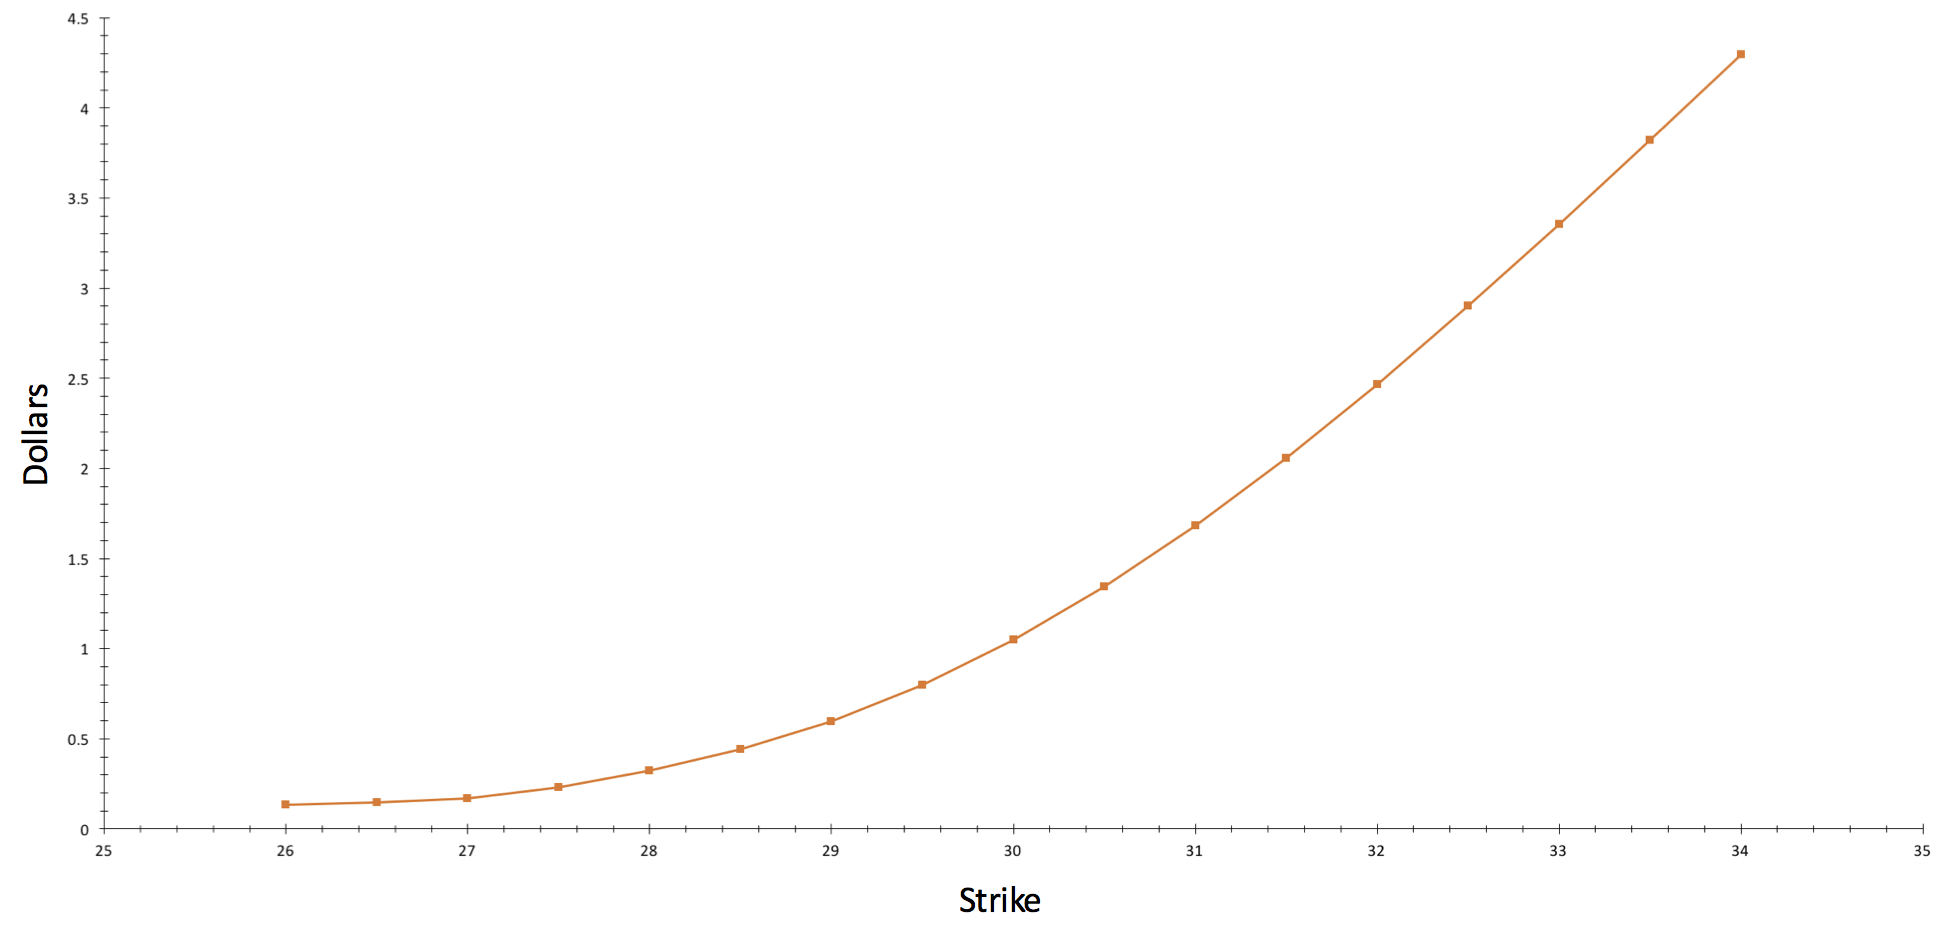
\includegraphics[width=1\textwidth]{Example_Call_Price_Plot}}
\end{figure}

If one were to calculate the volatilities given the above prices, the resulting plot would look like:

\begin{figure}[H]
	\caption{Example Intra-Expiration Call Volatilities By Strike}
	\centerline{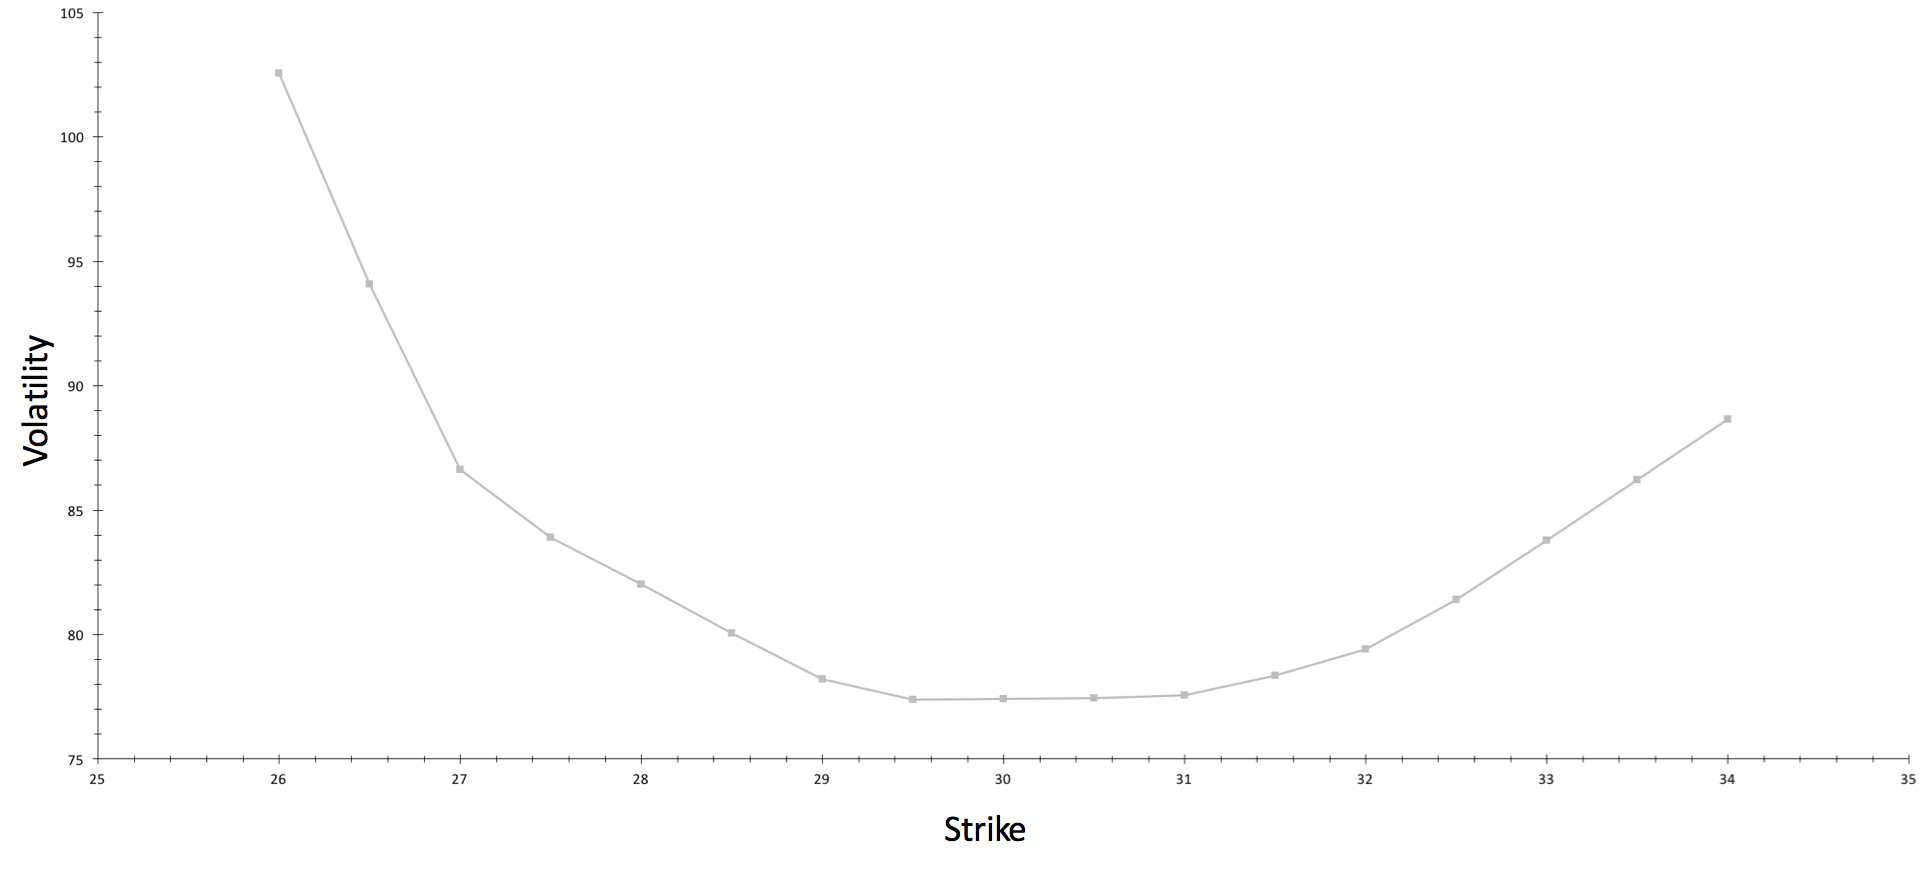
\includegraphics[width=1\textwidth]{Example_Call_Vol_Plot}}\label{fig:ExCallVolsByStrike}
\end{figure}

From figure \ref{fig:ExCallVolsByStrike}, it should be clear why it is colloquially called a smile\footnote{Sometimes an option's expiration is set close to an underlying asset's earnings announcement date.  In this scenario (and possibly others), as the expiration date (and earnings announcement) draw nearer, the `smile' can in fact turn into a `frown'.}.
\newpar
This project includes an analysis of various ways one can parameterize, optimize, and utilize the volatility smile.  In particular, it provides a start-to-finish approach for creating nonlinear least-squares optimized volatilities and making automated trading decisions from those theoretical values.
\newpar
The volatility smile is heavily relied upon in the world of options trading.  Often, a trader may have a handful of automated algorithms working rapidly and simultaneously\footnote{A typical algorithm can make a trading decision on the order of microseconds or better.  In many cases, nanoseconds. The utilization of Field Programmable Gate Arrays (FPGA's) is typically required to acheive such processing speeds.}.  These algorithms depend on the theoretical value for the option, which depends directly on the volatility that the trader has set for the option.  The volatility is typically set through an optimization process, given that there are thousands of options spanning multiple stocks that the trader will trade at once.

\newpage
\section{Introduction} \label{sec:Introduction}
This project provides a practical analysis of modeling what is known in options trading as the volatility smile.  In particular, how a chosen functional form, optimization process, and trading style can potentially affect a firm's profit or loss.  There are a number of papers that discuss how to model the volatility smile, but few present the practical implications of a particular model choice.  Moreover, even fewer papers discuss in detail the nontrivial and equally important steps of market data collection, filtering, and processing.  It is in this project that all steps of the process are examined;  from the collection of the market data to the resulting theoretical values and how each step in the entire process can affect a trading firm's bottom line.
Without this analysis, it is not immediately clear how a single choice in any one part of the process can cause an arbitrage-free set of market data to yield an arbitrage-full set of theoretical values.
\newpar
Although there are many types of financial derivatives to choose from, the scope of this paper covers only that of American Options on American Equities.  The reasoning for this decision is two-fold: the data are readily available, and years of working in a small trading prop shop that handles this derivative allows me to speak empirically on many of the concepts.  While it may be possible to apply the concepts here to other derivatives such as the European Option or American Options on other assets besides American Equities, lack of explicit experience lends caution from commenting on them.
\newpar
This project examines options on two American equities.  For every expiration date for both equities, a unique combination of parameterization, weighting scheme, and trading paradigm are chosen.  Then, at one-minute intervals throughout a single trading day, each combination is simulated from start to finish.  The results are analyzed and discussed here.
\newpar
By construction, the project setup results in a large number of simulations.  To simplify and streamline the analysis process, two C\# software programs were written: one to save market data and trader inputs to a set of files, and the other to run simulations from those inputs.
\newpage
\section{Methods}
Once a particular stock, expiration, volatility smile parameterization, weighting scheme, and trading strategy are chosen, the complete start-to-finish analysis of the volatility smile requires three steps:
\begin{enumerate}
	\item Gather and process the market data.  Market data can often be `noisy', and multiple snapshots of the same dataset should be gathered throughout the desired timeframe.  Additionally, the data must be converted from market prices into volatilities for future analysis.  See section \ref{subsec:MarketDataProcessing} for details.  \label{Analysis:MktDataProcessingStep}
    \item Find the least-squares fit of the volatility data given the chosen model and chosen weighting scheme for each market data snapshot in step \ref{Analysis:MktDataProcessingStep}.  Accomplishing this requires the implementation of a numerical optimization algorithm.  The algorithms utilized in this project are discussed in section \ref{subsec:NonlinearLeastSquaresOptimization}.\label{Analysis:RunOptimizationStep}
    \item Run a trading simulation given the chosen trading strategy, optimized data from step \ref{Analysis:RunOptimizationStep}, and the raw unfiltered market data.  Trading strategies and implementation details are outlined in section \ref{sec:TradingStrategies}.
\end{enumerate}
Specific details on the above three step process are discussed in the following subsections.

\subsection{Market Data Processing}
\label{subsec:MarketDataProcessing}
The importance of the infrequently discussed process of gathering and filtering the market data can be captured with the aphorism `garbage in, garbage out'.  Simply put, even the most superior models will produce poor results if the data given to it has not been properly vetted.  This section briefly discusses the details on how data were gathered and filtered prior to the parameterization and optimization processes.

\subsubsection{Collection of Data}\label{sec:CollectionOfData}
For this project, market data snapshots were collected\footnote{A separate C\# program was written which queried a third-party API provided by MayStreet, LLC.  Their website is http://www.maystreet.com/.  For a free source of option data, one can go to http://www.cboe.com/, the main website for the Chicago Board of Options Exchange.} every minute on Monday, February 12\textsuperscript{th}, 2018 for all the expiration dates provided by the CBOE for the stocks NVDA and TSLA.  Once the data were obtained, they were saved into separate files for each underlying asset in Java Standard Object Notation (JSON) format.
\newpar
For each underlying asset, data collected include:
    \begin{enumerate}
    	\item	The National Best Bid and Offer (NBBO) prices for each listed option.
        \item	The bid and ask prices of the underlying asset (the stock price).
        \item	A set of expected or announced future dividends, if any.
        \item	The carry and premium rates for each expiration, chosen to best `line up'\footnote{`line up' here comes from the theory that the at-the-money call and put prices must be equivalent.  Thus, it is possible to find a carry rate that best makes the at-the-money call and put theoretical values equal.  There are some cases where the trader will intentionally choose an incorrect carry rate in order to help drive his algorithms to develop a particular position.} the option board.
        \item	Time to expiration that accounts for trading time and holidays.
    \end{enumerate}
    
\subsubsection{Converting to Volatility}\label{sec:ConvertingToVol}
A proprietary variation of a trinomial lattice based option pricing model was chosen for this project.  This was done for two reasons: to ensure accuracy and direct applicability of the results to the trading paradigms of my current employer, and because writing an American Option pricing model from scratch is beyond the scope of this project.  To convert to and from option theoretical value and volatility, this particular model requires the inputs of strike, option type (put or call), time to expiration (in years), price of the underlying asset (here, the NBBO midpoint was used), the expiration's carry and premium rates, and dividends (if any).

\subsubsection{Filtering Methods}\label{sec:FilteringMethods}
Once the four sets of call bid, call ask, put bid, and put ask implied volatility (IV) per strike per expiration were obtained, a significant amount of filtering and processing is required to produce a single set of strike-volatility data points.  This filtering process utilized three algorithms:

\begin{enumerate}
	\item \textbf{GetBestBidAskIvMarket}:  This method converts the four-fold dataset of (Strike, CallBidIv, CallAskIv, PutBidIv, PutAskIv) into the two fold (Strike, BidIv, AskIv), an option type-independent dataset.  ``Best'' here is defined as the IV which yields the BidIv and AskIv pair which are closest to each other, i.e. the `tightest' market.  This method uses the algorithm's AdjustRawBidIvs and AdjustRawAskIvs.  Additionally it prevents strikes that have sparse data or volatility calculation errors from being included in the input data that is passed to the optimization algorithm.
    \item \textbf{AdjustRawBidIvs}: This algorithm attempts to prevent BidIvs that are theoretically impossible, or volatilities that could be used to arbitrage the market.  In words: make sure that as you go away from at-the-money, no BidIv is smaller than the surrounding strike's Bid IV's.  If you find an IV where the IV at the previous strike AND next strike are both greater than it, then modify that IV to be linearly interpolated between the surrounding strikes' IV's.  Repeat until there are no more places to interpolate or until you have exceeded five seconds of computation time.
    \item \textbf{AdjustRawAskIvs}:  This algorithm also attempts to prevent AskIvs that are theoretically impossible, or volatilities that could be used to arbitrage the market.  In words: Make sure that as you go away from at-the-money, no AskIv is bigger than it's surrounding strikes Ask IV's.  If you find an IV where the IV at the previous strike AND next strike are both less than it, then modify that IV to be linearly interpolated between its surrounding strikes' AskIvs.  Repeat until there are no more places to interpolate or until you have exceeded five seconds of computation time.
\end{enumerate}

\subsection{Volatility Smile Parameterizations}\label{sec:VolSmileParameterizations}
In order for a parameterization to be successful in a trading environment, it must first and foremost fit the volatility data closely.  That is, it must closely match a set of $N$ known strike-volatility pairs $\{(k_i,\sigma_i) \ ; \ i = 1,2,\cdots,N\}$, with $N$ typically being less than 100.
If one has a bad parameterization, then both the trader and their automated trading algorithms will be poorly informed when making trading decisions.  To illustrate this fact, the following parameterizations are examined in this project.

\subsubsection{Basic Parameterizations}\label{subsec:BasicParameterizations}
Let $\Sigma(k)$ be the function of volatility with respect to strike $k$.  Then we define the following three basic volatility smile parameterizations:
\begin{enumerate}
	\item \textbf{Raw Filtered Mid-Market}
    \newline Simply use the non-optimized but filtered mid-market implied volatility for each strike.  This is the equivalent of a cubic spline that goes through each point and serves as a control group.
    \item \textbf{Linear} 
    \newline A basic linear parameterization $\Sigma(k) = bk + a$, with parameters $a,b$.  This clearly is a terrible parameterization of the volatility smile, but helps highlight exactly how a bad model can affect the overall profit and loss.
    \item \textbf{Quadratic}
    \newline A simple quadratic parameterization $\Sigma(k) = ck^2 + bk + a$, with parameters $a,b,c$.  It is not completely obvious that this parameterization does a poor job modelling the volatility smile.  In particular though, strikes around at the money may look good but as you go out of the money you run into trouble.
\end{enumerate}

\subsubsection{Elasticity Inspired}\label{subsec:ElasticityParameterizations}
The following elastic smile parameterizations attempt to define a function that is not only a smooth, close fit of the data, but also provide additional information to the trader about the general shape of the volatility smile.  Essentially we have attempted to build in `trading sense' into the function - i.e. the volatilities that the parameterization produces are ones that are sensible from trader's point of view (no arbitrage violations...etc).
\newpar
When we talk about `trading sense', we are discussing how a non-mathematical observer sees and processes the data.  First, the volatility smile is visibly both continuous and smooth.  Second, a percentage change from the at-the-money strike to one higher should have the same percentage change as from the at-the-money strike to one lower.  Third, there is a notion of elasticity of volatility with respect to strike, as well as a feeling of a recursive relationship where the elasticity of volatility itself has some elastic behavior with respect to strike.
\newpar
The elastic smile incorporates the notion of elasticity of volatility with respect to strike; that is, the percentage change in volatility relative to the percentage change in strike.  This elasticity is referred to as the `skewness', and is measured at the forward price, or the at-the-money portion of the volatility smile.  The elasticity of the skewness is referred to as the `curvature', and the elasticity of the curvature is referred to as the `twist'.  Mathematical derivations of the first and second order elastic smile parameterization schemes are provided in appendix \ref{appendix:ElasticSmileDerivation}.
\newpar
Again let $\Sigma(k)$ be the function of volatility with respect to strike price $k$, $\sigma_f$ be the volatility at the forward price $f$, and $n(k)$ be the percentage change from the forward price for a given strike $k$.  By definition,
\begin{equation*}
n(k) = 	\begin{cases}
			n_L(k) = \frac{100\left(f-k\right)}{f} & \mathFor k < f\\
            n_R(k) = \frac{100\left(k-f\right)}{f} & \mathFor k \geq f\\
		\end{cases}.
\end{equation*}
To simplify our elasticity-based parameterizations, we will instead define $n(k)$ to be negative for strikes above the forward price, thus simplifying $n(k)$ to be

\begin{equation*}
	n(k) = 	\frac{100\left(f-k\right)}{f} \ \forall k.
\end{equation*}

The elastic smile parameterizations are then given by:

\subsubsection*{First Order (Skew Only)}
\begin{equation}
	\Sigma(k) = \sigma_f\mathbb{S}^{n(k)} \label{FirstOrderSmile},
\end{equation}
where $\sigma_f$ (forward volatility) and $\mathbb{S}$ (Skew) are the only parameters.

\subsubsection*{Second Order (Skew and Curvature)}

\ifhidesecrets

\begin{equation}
[Omitted],
\label{SecondOrderSmile}
\end{equation}

\else

\begin{equation}
\Sigma(k) = \begin{cases}
			\sigma_f\left(\mathbb{S}\right)^{n(k)}\left(\mathbb{C}_l\right)^{n^{2}(k)} & \mathFor k < f	\\
            \sigma_f\left(\mathbb{S}\right)^{n(k)}\left(\mathbb{C}_r\right)^{n^{2}(k)} & \mathFor k \geq f	\\
        \end{cases},
\label{SecondOrderSmile}
\end{equation}

\fi

with $\sigma_f$, $\mathbb{S}$, $\mathbb{C}_l$ (Left Curvature), and $\mathbb{C}_r$ (Right Curvature) as parameters.

\subsubsection*{Third Order (Skew, Curvature, and Twist)}
\begin{equation}
\Sigma(k) = \begin{cases}
			\sigma_f\left(\mathbb{S}\right)^{n(k)}\left(\mathbb{C}_l\right)^{n^{2}(k)}\left(\mathbb{T}_l\right)^{n^{3}(k)} & \mathFor k < f	\\
            \sigma_f\left(\mathbb{S}\right)^{n(k)}\left(\mathbb{C}_r\right)^{n^{2}(k)}\left(\mathbb{T}_r\right)^{n^{3}(k)} & \mathFor k \geq f	\\
        \end{cases},
\label{ThirdOrderSmile}
\end{equation}
with $\sigma_f$, $\mathbb{S}$, $\mathbb{C}_l$, and $\mathbb{C}_r$, $\mathbb{T}_l$ (Left Twist), and $\mathbb{T}_r$ (Right Twist) as parameters.

\subsubsection{Natural Log Modification to the Elastic Smile Parameterizations}
\label{subsec:NatLogElasticMod}
A keen mathematical mind may notice that the first, second, and third order elastic smile parameterizations may have poor numerical properties.  In particular, it is usually the case that $\mathbb{S} \approx 1$ and $n(k)$ is quite large - on the order of 1000 or more in many cases.  For the $\mathbb{C}_l$ and $\mathbb{C}_r$ parameters, the poor numerical properties are even further exacerbated since we raise each to the power of $n^{2}(k)$ and it is usually the case that $1 < \mathbb{C}_{l,r} < \mathbb{S}$.  The bad numerical properties are even more exacerbated with the twist parameters $\mathbb{T}_{l}$ and $\mathbb{T}_{r}$, since we raise both to the $n^{3}(k)$ power and usually $1 < \mathbb{T}_{l,r} < \mathbb{C}_{l,r}$.  On top of all that, everything is multiplied together with the goal of obtaining a value that is usually between zero and one.
\newpar
One way to potentially improve the numerical properties of the elasticity inspired parameterizations is to instead analyze the natural log of the volatility smile, and then convert back to normal volatility once the optimization is complete.  Making this change to the second order elastic smile gives:
\begin{align*}
\ln(\Sigma(k)) 
&= 		\begin{cases}
			\ln\left(\sigma_f\left(\mathbb{S}\right)^{n(k)}\left(\mathbb{C}_l\right)^{n^{2}(k)}\right) & \mathFor k < f	\\
            \ln\left(\sigma_f\left(\mathbb{S}\right)^{n(k)}\left(\mathbb{C}_r\right)^{n^{2}(k)}\right) & \mathFor k \geq f	\\
        \end{cases} \\
&=		\begin{cases}
			\ln(\sigma_f) + n(k)\ln(\mathbb{S}) + n^{2}(k)\ln(\mathbb{C}_l) & \mathFor k < f	\\	
            \ln(\sigma_f) - n(k)\ln(\mathbb{S}) + n^{2}(k)\ln(\mathbb{C}_r) & \mathFor k \geq f	\\
        \end{cases}, \numberthis
\end{align*}
\label{SecondOrderSmileNaturalLog}
\newline
which eliminates the troublesome numerical properties of equation \ref{SecondOrderSmile}.  A similar transformation can also be performed for the first and third order smile parameterizations, but only the modification to the second order is discussed in section \ref{subsec:AddressingNumericalConcerns}.
\subsubsection{Other Parameterization Methods}
There are also a number of publicly available optimization styles and parameterizations available to model the volatility smile.  Other methods are not included in the analysis here, but for the curious reader, a few notable ones are named below.
\begin{enumerate}
	\item A stochastic-volatility inspired parameterization provided by Jim Gatheral\textsuperscript{\cite{Gatheral}}:
\begin{equation}
\Sigma^{2}(k) = a + b\Big\{p(k-m) + \sqrt{(k-m)^{2}+ \sigma^{2}} \Big\},
\end{equation}
where $\Sigma(k)$ is the volatility as a function of strike $k$ (for a single expiration and underlying asset), and $\{a,b,p,m,\sigma\}$ are fitting parameters.
	\item Roger Lee's moment formula for extreme strikes\textsuperscript{\cite{Lee}}.
    \item Matthias R. Fengler's arbitrage free smoother\textsuperscript{\cite{Fengler}}, notably NOT a parameterized curve but instead a smoothing algorithm with constraints that force it to be arbitrage-free in terms of option trading.
\end{enumerate}

\subsection{Weighting Schemes}\label{sec:WeightingSchemes}
From a trading standpoint, not all strikes are created equal.  It is important to communicate to the optimization process which points are more important than others.  In general, strikes closer to the forward price are more important to a trader than the further in-the-money or out-of-the-money strikes.  One way to communicate strike importance to least-squares optimization algorithm is to incorporate a weighting number for each data point.  The following weighting styles were examined for this project:

\begin{enumerate}
	\item \textbf{Evenly Weighted} (Even) \newline This is equivalent to an unweighted optimization process.  Each (Strike,Volatility) pair in the dataset is given an equal weight of $1$.
    \item \textbf{Raw Volatility Width} (VW) \newline This weights each (Strike,Volatility) point proportionally based on the point's filtered market Bid/Ask Iv spread relative to the average filtered market Bid/Ask Iv spread for the entire expiration dataset.
    \item \textbf{Volatility Width Vega Multiplier} (VWVM) \newline This weights each (Strike, Volatility) point based on the (filtered) market Bid/Ask Iv spread along with a multiplier related to the corresponding vega for each strike.  The vega for each strike is determined using the same pricing model as described in \ref{sec:ConvertingToVol}
    \item \textbf{Volatility Width Vega Multiplier Squared} (VWVM\textsuperscript{2}) \newline Equal to the square of the Volatility Width Vega Multiplier.
    \item \textbf{Square Root Volatility Width Vega Multiplier} ($\sqrt{\text{VWVM}}$) \newline Equal to the square root of the Volatility Width Vega Multiplier.
\end{enumerate}

\subsection{Nonlinear Least Squares Optimization}
\label{subsec:NonlinearLeastSquaresOptimization}
The retrieved option data, once processed (section \ref{sec:CollectionOfData}), provides a set of $N$ strike-volatility pairs $\{(k_i,\sigma_i) \ ; \ i = 1,2,\cdots,N\}$.  We then pick a function $f(k,\lambdaVect)$ to model the $N$ data points\footnote{Typically, $N < 100$}.  Here, $\lambdaVect = [\lambda_1, \lambda_2, \cdots, \lambda_M]^T$ is a $1 \times M$ vector of parameters $(M < N)$ for the function $f(k,\lambdaVect)$, with $k$ being an independent variable.  Then the error at the $i^{th}$ strike $k_i$ is $r_i = \sigma_i - f(k_i, \lambdaVect)$, where $\sigma_i$ is the input volatility at $i^{th}$ strike.
\newpar
The goal of any least-squares optimization process is then to find the $M$ parameter values of $\lambdaVect$ that minimize the sum of squared errors.  In other words, we want to find $\lambdaVect$ so that the following function is minimized:
\begin{equation}
	F(\lambdaVect) = \sum_{i=1}^{N}(\sigma_i - f(k_i,\lambdaVect))^2 = \sum_{i=1}^{N}r_i^2.
    \label{eq:LeastSquaresF}
\end{equation}
Additionally, a weighting factor can easily be applied for each data point.  Let the weighting factor for the $i^{th}$ data point be denoted as $w_i$.  Then equation \ref{eq:LeastSquaresF} becomes
\begin{equation}
	F(\lambdaVect) = \sum_{i=1}^{N}(\sigma_i - f(k_i,\lambdaVect))^2w_i = \sum_{i=1}^{N}r_i^2w_i.
    \label{eq:LeastSquaresFWeighted}
\end{equation}

This project requires obtaining a parameter vector $\lambdaVect$ that minimizes equation \ref{eq:LeastSquaresFWeighted}.  In the case of a linear $f(k,\lambdaVect) = ak + b$ parameterization and even weighting scheme, for example, we will have $\lambdaVect = (a, b)^T$ and $w_i = 1 \enskip \forall \enskip i = 1, \cdots, N$.
\newpar
Now, let $\pmb{\sigma} = [\sigma_1, \sigma_2, \cdots, \sigma_N]^T$ and
    $\pmb{f}(\lambdaVect) = [f(k_1,\lambdaVect), f(k_2,\lambdaVect)\cdots, f(k_N,\lambdaVect)]^T$.  Then it follows that $\pmb{r}(\lambdaVect) = \pmb{\sigma} - \pmb{f}(\lambdaVect)$ and from equation \ref{eq:LeastSquaresFWeighted},
\begin{equation}
    F(\lambdaVect) = (\pmb{\sigma} - \pmb{f}(\lambdaVect))^T W (\pmb{\sigma} - \pmb{f}(\lambdaVect)) = \pmb{r}(\lambdaVect)^T W \pmb{r}(\lambdaVect).
    \label{eq:LeastSquaresFWeightedMatrix}
\end{equation}
Where $W$ is a diagonal $N \times N$ matrix with $W_{ii} = w_i$.  Note that modelling the option volatility smile for practical purposes has empirically required some set of nonuniform weighting factors $w_i$.
\newpar
Two algorithms for least squares optimization are compared for each of the chosen parameterization schemes in section \ref{sec:VolSmileParameterizations}:  The Gauss-Newton and Levenberg-Marquardt algorithms\footnote{Note that the algorithms were designed for use with dense datasets such as the option volatility smile, and does not take advantage of any sparsity arguments that can often be made when solving other problems in optimization.}.  Both algorithms were arbitrarily chosen to stop when the difference between the sum of least squares from the previous step to the current step was less than $10^{-14}$ in magnitude\footnote{At $10^{-14}$ (and even greater), further adjustments yield little to no difference in the resulting theoretical values and thus no notable difference for practical use.}.
\newpar
The freely available Math.Net Numerics library\footnote{https://numerics.mathdotnet.com/} for C\# was utilized for necessary linear algebra computations.  This allowed focus to remain on the optimization algorithm and avoided the unnecessary re-creation of already established and well-known algorithms in linear algebra.

\subsubsection{Gauss-Newton and Levenberg-Marquardt}\label{subsubsec:GNLM}

Since most of the model functions analyzed in this project are nonlinear, the minimization of $F(\lambdaVect)$ was carried out in an iterative manner using either the Gauss-Newton or Levenberg-Marquardt process\footnote{The Gradient Descent method was also explored, but this algorithm proved to be much, much slower than the Gauss-Newton and Levenberg-Marquardt and required constant adjustment to its input settings (like step size) for each data set.  For these reasons it was deemed unfit for practical use in a trading environment and thus left out of this project}.  The goal for either algorithm at each step is to find a `step' vector $\pmb{\eta}$ such that $F(\lambdaVect + \pmb{\eta}) < F(\lambdaVect)$.  In other words, so that the resulting sum of least squares is reduced after the step\textsuperscript{\cite{Gavin}}.
\newpar
For the outlines of both optimization algorithms, we define the following:
\begin{itemize}
\item $s$ as current step number in the iteration 
\item $J$ as the $N \times M$ Jacobian matrix of the function $f(k,\lambdaVect)$.  That is, 
\begin{equation*}
	J_{ij} = \frac{\partial f(k_i,\lambdaVect)}{\partial \lambda_j}, \quad i = 1,\cdots, N \quad \text{and} \quad j = 1,\cdots, M.
\end{equation*}
\item $\lambdaVect_s$ as the approximate solution vector at step $s$
\end{itemize}

\textbf{\underline{The Gauss-Newton Algorithm}}
\newline
From \cite{Gavin}, the step vector at each step for the Gauss-Newton method can be found by solving 
\begin{equation}
    (J^T W J) \pmb{\eta} = J^T W (\pmb{\sigma} - \pmb{f}(\lambdaVect))
\end{equation}
for the vector $\pmb{\eta}$.  Pseudocode for the C\# implementation of this algorithm is as follows\footnote{Note that all matrix algebra was performed using the Math.Net Numerics library (https://numerics.mathdotnet.com/)}:
\begin{enumerate}
	\item Set $s = 0$ and $\lambdaVect_s = \lambdaVect_0$
    \item while $s < maxSteps$
      \begin{enumerate}
          \item $\pmb{d} = \pmb{\sigma} - \pmb{f}(k,\lambdaVect_{s})$
          \item Calculate $J$ from $\pmb{f}(k,\lambdaVect_{s})$
          \item Solve $(J^T W J) \pmb{\eta} = J^T W \pmb{d}$ for $\pmb{\eta}$
          \item $\lambdaVect_{s+1} = \lambdaVect_{s} + \pmb{\eta}$
          \item $stop = (|F(\lambdaVect_{s}) - F(\lambdaVect_{s+1})| \leq 10^{-14})$
          \item $\lambdaVect_{s} = \lambdaVect_{s+1}$
          \item $s = s + 1$
          \item If $stop$, break out of the loop and go to step \ref{GN_CalcR2}.
      \end{enumerate}
    \item Calculate the coefficient of determination ($R^2$).\label{GN_CalcR2}
\end{enumerate}

\textbf{\underline{The Levenberg-Marquardt Algorithm}}
\newline
The Levenberg-Marquardt algorithm in this project was adapted directly from Levenberg \cite{Levenberg} and Marquardt \cite{Marquardt}.  From Marquardt, the step $\pmb{\eta}$ to compute the parameter vector $\lambdaVect$ at each step is given by solving
\begin{equation}
    (J^T W J + \kappa I)\pmb{\eta} = J^T W (\pmb{\sigma} - \pmb{f}(k,\lambdaVect_{s})),
    \label{eq:LevenbergUpdate}
\end{equation}
where $I$ is the identity matrix.  The parameter $\kappa$ allows the algorithm to update $\lambdaVect$ with a combination of both a Gauss-Newton step and a steepest descent step.  For small $\kappa$, the step vector $\pmb{\eta}$ results in a Gauss-Newton update.  For large $\kappa$, the step $\pmb{\eta}$ results in a Gradient Descent update\textsuperscript{\cite{Gavin}}.
\newpar
Fletcher (\cite{Fletcher}) proposes a modification to the algorithm that replaces the identity matrix $I$ in equation \ref{eq:LevenbergUpdate} with a diagonal matrix consisting of the diagonal elements of $J^T J$.  This modification is utilized in this project, and causes equation \ref{eq:LevenbergUpdate} to become
\begin{equation}
    (J^T W J + \kappa \; \text{diag}(J^T W J))\pmb{\eta} = J^T W (\pmb{\sigma} - \pmb{f}(k,\lambdaVect_{s})).
    \label{eq:MarquardtUpdate}
\end{equation}
Once an initial value for $\kappa$ is chosen\footnote{For this project, the initial value was chosen to be $\kappa = 0.01$}, a decision must then be made on how to update this parameter at each step.  While there are many papers discussing methods to update $\kappa$, the update strategy used here follows directly from Marquardt (\cite{Marquardt}).
\newpar
Let $\Phi(\kappa_s)$ be the sum of squares at step $s$ after applying equation \ref{eq:MarquardtUpdate} with $\kappa = \kappa_s$.  Let $\rho > 1$ be some constant\footnote{Fixing $\rho = 2$ seemed to suffice for all datasets analyzed here.}.  Then at each next step $s + 1$, $\kappa_{s + 1}$ is determined by the following process:
\begin{itemize}
    \item If $\Phi( \frac{\kappa_{s}}{\rho}) \leq \Phi(\kappa_{s})$, then $\kappa_{s+1} = \frac{\kappa_{s}}{\rho}$.
    \item Else find the minimum integer $w \geq 1$ such that $\Phi(\kappa_s \rho^w) \leq \Phi(\kappa_{s})$.  Then $\kappa_{s+1} = \kappa_s \rho^w$.
\end{itemize}

Pseudocode for the implementation of the Levenberg-Marquardt algorithm is as follows\footnote{Again, note that all matrix algebra was performed using the Math.Net Numerics library (https://numerics.mathdotnet.com/)}:
\newpage
\begin{enumerate}
	\item $\kappa = 0.01$, $\rho = 2.0$, $\lambdaVect_s = \lambdaVect_0$
	\item while $s < maxSteps$
    	\begin{enumerate}
        	\item $\pmb{d} = \pmb{\sigma} - \pmb{f}(k, \pmb{\lambda}_{s})$
            \item Calculate $J$ from $\pmb{f}(k, \pmb{\lambda}_{s})$
            \item $\kappa = \frac{\kappa}{\rho}$
            \item Solve $\left(J^{T} W J + \kappa \; \text{diag}(J^{T} W J)\right) \pmb{\eta} = J^{T} W \pmb{d}$ for $\pmb{\eta}$
            \item $\lambdaVect_{s+1} = \pmb{\lambda}_{s} + \pmb{\eta}$
            \item while $F(\lambdaVect_{s+1}) > F(\pmb{\lambda}_{s})$
                    \begin{enumerate}
                        \item $\kappa = \rho \kappa$              
                        \item Solve $\left(J^{T} W J + \kappa \; \text{diag}(J^{T} W J)\right) \pmb{\eta} = J^{T} W \pmb{d}$ for $\pmb{\eta}$
                        \item $\lambdaVect_{s+1} = \pmb{\lambda}_{s} + \pmb{\eta}$
                    \end{enumerate}
            \item $stop = (|F(\lambdaVect_{s}) - F(\lambdaVect_{s+1})| \leq 10^{-14})$
            \item $\pmb{\lambda}_{s} = \lambdaVect_{s+1}$
            \item $s = s + 1$
            \item If $stop$, break out of the loop and go to step \ref{LM_CalcR2}
    	\end{enumerate}
   \item Calculate the coefficient of determination ($R^2$). \label{LM_CalcR2}
\end{enumerate}

\subsection{Trading Simulations}\label{sec:TradingStrategies}
One end goal of this project is to show how both good and bad parameterizations of the volatility smile can affect a trader's profit or loss.  Illustrating this point requires both well-defined parameterizations and a handful of trading simulations that reasonably represent potential real-world trading algorithms.  A trading simulation in this project consists of four pieces: the actual trading strategy, a scope on what it is allowed to trade, imposed limits to simulate risk exposure, and a timeframe for which to execute the simulations.

\subsubsection{Strategies And Scope}
\label{subsec:TradingStrategiesAndScope}
Each of the trading strategies analyzed in this project were based on the concept of trading edge.  We define \textit{trading edge} as the dollar difference between an option's theoretical value and the corresponding bid or ask market price.  For example, suppose an option has a market bid price of \$0.85 and a market ask price of \$1.10.  If the option's theoretical value is evaluated to be \$1.00, then we say the theoretical value has 15 cents of edge with respect to the bid price and 10 cents of edge with respect to the ask price.  If the theoretical value falls below the market bid price or above the market ask price, it is said to have `crossed' the market and thus will have a negative edge.
\newpar
The concept of edge need not be limited to precise dollar amounts.  It can also be expressed as the percent of edge relative to the total market width.  For example, if an option market quote is currently \$1.00 bid and \$2.00 offered, then a theoretical value of \$1.35 will have 35\% edge relative to the bid and 65\% edge relative to the offer\footnote{The market width is \$1.00, thus \$1.35 is 35\% above the bid and 65\% below the ask price}.  Both raw dollar edge and percent-edge trading strategies are analyzed in this project.  This project examined trading strategies within the edge ranges of $[-\$0.15, \$0.15]$ and $[-15\%, 15\%]$.
\newpar
The analyzed trading strategies each evaluate the theoretical edge and make trades on a single option-by-option basis rather than groups of options.  It is not uncommon to have trading strategies that trade specific groups of options at a time such as straddles, butterflies, or any other intra-expiration spread.  This added unnecessary complexity to the project and has been left out of the analysis here.
\newpar
It is possible to encounter situations where the market quote provides fewer contracts than one would like to trade.  If only four contracts are available for a particular side of the market for example, then clearly one cannot trade more than four on that line.  Some real-world trading strategies may take the size of the market quote into account when determining whether or not to make a trade.  This type of analysis - trading based on available market size - is left out of this project.  All trading algorithms utilized in this project trade any available market size up to a maximum quantity of ten per trade.  In other words, if the market size is less than ten, the trading simulation will trade the number of available contracts.
\newpar
Finally, we limit each trading simulation to only make trades within the domain of a single expiration for a single underlying asset.  More complex trading strategies exist such as time spreads (inter-expiration) or spreads between stocks.  Such trading strategies go beyond the scope of this project.

\subsubsection{Risk Exposure And Time Frame}
\label{subsec:RiskExposureAndTimeFrame}
Without imposing limits on how much a trading simulation is allowed to trade, it is quite possible that the simulation establishes an unrealistic position that is far beyond any normal risk tolerance.  To provide risk limits, a notion of `delta exposure' is introduced to each trading simulation.  In the trading world, the option's delta can provide a (\textit{very}) rough guideline for the required quantity of underlying shares that need to be traded (`hedged') to offset the option's purchase or sale.  Here, the delta is used to approximately gauge the number of underlying shares a particular trading simulation is long or short.  If the simulation desires to make a trade it must first check to see if the trade would create a new positional delta that would be beyond the allowed limits.  To keep things as simple as possible, all analyzed trading simulations adhere to an upper delta exposure limit of 1,000 and a lower delta exposure limit of -1,000.  In other words, the trading simulations must not have a position that is long or short more than approximately 1,000 shares of the corresponding stock.
\newpar
Finally, trading simulations are allowed to make trades at one-minute intervals throughout the trading day, starting one minute after market open and ending one minute before market close.

\subsection{The Analysis Program}
The data are analyzed with the help of a custom-written C\# program that reads saved data files from a particular folder and allows simulations to run on any combination of stock, expiration, fit parameterization, weighting scheme, and trading style desired for the given dataset.
\newpar
The reason for creating an entire software program to run simulations is due to the sheer amount of data to analyze.  Suppose we wanted to run a simulation for just a single expiration date for a single stock, five different parameterization schemes, two different optimization algorithms, five different trading strategies, and at one-minute trading intervals.  This would mean that for each data snapshot at each trading interval there are $5 \times 2 \times 5 = 50$ combinations of expiration, parameterization, and trading scheme to analyze.  At one minute trading intervals, we take 388 data snapshots in a single trading day, creating a set of $388 \times 50 = 19,400$ simulations per day to be run.
\newpar
At the surface, the software program performed the following steps on the data provided to it:
\begin{enumerate}
	\item For a given stock and expiration, group the data into unique combinations of optimization algorithm, weighting scheme, and trading style.\label{item:GroupData}
    \item For every data set matching the underlying and expiration date chosen in step \ref{item:GroupData}, process the market data by
    \begin{enumerate}
    	 \item Converting each option's bid and ask price into volatilities (section \ref{sec:ConvertingToVol}).
         \item Filtering the data into a single set of $(strike, volatility)$ data points (section \ref{sec:FilteringMethods}).
         \item Ordering this single set of volatility data by strike from least to greatest.
         \item Trimming data from the ends of the data domain (section \ref{sec:FilteringMethods}).\label{item:FilterConvertTrim}
    \end{enumerate}
	\item Group and order the data in step \ref{item:FilterConvertTrim} by date collected.  Run a nonlinear least-squares optimization process for the chosen parameterization and weighting schemes.  Record the current option position and simulate trades based upon a chosen trading strategy.
   \item Create an excel document with results and statistics.
\end{enumerate}

The above results in the analysis of unique combinations of: underlying asset, expiration date, parameterization function, weighting scheme, and trading strategy.  Since there is far too much data to analyze here, only a smaller subset of results is presented.

\subsection{Summary of Project Scope}
The end project scope was eventually downsized from the original goal in an effort to simplify the analysis of the simulations. The scope included all combinations of the following:

\begin{enumerate}
    \item American option market data collected on one-minute intervals on Monday, February 12\textsuperscript{th} 2018
    \begin{enumerate}
        \item NVDA Expirations:  3/16/18, 6/15/18, 1/18/19
        \item TSLA Expirations:  3/16/18, 4/20/18, 1/18/19
    \end{enumerate}
    \item Volatility smile parameterizations
    \begin{enumerate}
        \item Basic (section \ref{subsec:BasicParameterizations}):  Raw, Linear, Quadratic
        \item Elastic (section \ref{subsec:ElasticityParameterizations}): Elastic, Smile, Twist
        \item Modified Elastic (section \ref{subsec:NatLogElasticMod}): Smile, Twist
    \end{enumerate}
    \item Nonlinear least squares optimization algorithms (section \ref{subsubsec:GNLM})
    \begin{enumerate}
        \item Gauss-Newton
        \item Levenberg-Marquardt
    \end{enumerate}
    \item Nonlinear optimization weighting schemes (section \ref{sec:WeightingSchemes}): Evenly, VolWidth, VolWidthVegaMult (VWVM), VWVM\textsuperscript{2}, $\sqrt{\text{VWVM}}$
    \item Trading strategies (section \ref{sec:TradingStrategies}):  Single-option edge strategies at quarter segments of $\pm0.15$ cents of edge and $\pm15$ percent width edge.
\end{enumerate}
Note that the above results in 39,110,400 separate simulations\footnote{Total of six expirations between two stocks, seven parameterizations, two optimization algorithms, five weighting schemes, 240 trading edge zones, 388 market data snapshots.  $6 \times 7 \times 2 \times 5 \times 240 \times 388 = 39,110,400$} (110,800 combinations for each snapshot).  This number can be reduced through the realization that simulations run using the Raw parameterization do not execute any optimization process, and thus many of the simulations will yield the same results, regardless of choice in optimization algorithm or weighting scheme.

\subsection{A Visual Example}
\label{sec:AVisualExample}
For the more visually inclined, let's consider options for TSLA that shared the same expiration date of March 16\textsuperscript{th}, 2018.  At about 11:45 AM CDT on February 12\textsuperscript{th}, 2018, the market prices are displayed in Figure \ref{fig:SampleOptMarketPrices}.  Since it is difficult to see the separation between the bid and ask prices on a plot, Table \ref{table:SampleOptionMarketDetail} shows the actual values around where the call and put prices cross. 

\img{TSLA 3/16/18 Midday Option Prices}{SampleOptionMarket}{fig:SampleOptMarketPrices}
\newpage
\begin{center}
  \captionsetup{hypcap=false}
  \captionof{table}{TSLA 3/16/18 Midday Option Price Detail}
  \begin{tabular}{ |>{\columncolor{Gray}}c|c|c|c|c| }
      \hline
      \rowcolor{LightCyan}
      \textbf{Strike} & \textbf{Call Bid} & \textbf{Call Ask} & \textbf{Put Bid} & \textbf{Put Ask} \\
      \hline
        300 &   \$22.40   &   \$23.00   &   \$11.05   &   \$11.35   \\  \hline
        305 &   \$19.30   &   \$19.80   &   \$12.95   &   \$13.25   \\  \hline
        310 &   \$16.64   &   \$17.05   &   \$15.15   &   \$15.45   \\  \hline
        315 &   \$14.15   &   \$14.45   &   \$17.60   &   \$17.95   \\  \hline
        320 &   \$12.00   &   \$12.15   &   \$20.25   &   \$20.70   \\  \hline
        325 &   \$10.05   &   \$10.15   &   \$23.25   &   \$23.60   \\  
      \hline
  \end{tabular}
  \label{table:SampleOptionMarketDetail}
\end{center}

Once the market data snapshot is obtained, each of the market prices are then put through the trinomial-lattice based pricing model to arrive at the volatilities in Figure \ref{fig:SampleOptionMarketIVs}.

\img{TSLA 3/16/18 Midday Market Volatilities}{SampleOptionMarketIVs}{fig:SampleOptionMarketIVs}

Note now that many points are now missing from the data, especially at the ends of the strike range.  The reason for this is embedded in the chosen option pricing model.  For the model used in this project, options with extremely low or zero price or options below parity can result in a zero-volatility output.  Recall that an option's value is typically made up of two components:  Intrinsic and Extrinsic value.  The former results from how the option contract is defined and it's strike price relative to the stock price.  The latter consists of other factors, of which the volatility can attribute to.  If for some reason the extrinsic value is zero as in the case of the below parity options, then there is essentially no volatility, and is thus missing from the plot in Figure \ref{fig:SampleOptionMarketIVs}.
\newpar
Converting the market prices into volatilities gives four sets of data for each strike:  Call Bid, Call Ask, Put Bid, and Put Ask implied volatility.  To be able to run a simple nonlinear least squares optimization process, the four data sets need to be condensed into a single set of data points.  The process by which this was accomplished is described in section \ref{sec:FilteringMethods}.  The result of which are shown in Figure \ref{fig:SampleInputIvs}.

\img{TSLA 3/16/18 Midday Input IVs}{SampleInputIvs}{fig:SampleInputIvs}

Plotted with the market implied volatilities shown in Figure \ref{fig:SampleOptionMarketIVs} gives the result in Figure \ref{fig:SampleInputIvsWithMarketIvs}.

\img{TSLA 3/16/18 Midday Input IVs with Market IVs}{SampleInputAndMktIVs}{fig:SampleInputIvsWithMarketIvs}

Next, we pick a parameterization, optimization algorithm, and weighting scheme.  For the Levenberg-Marquardt algorithm and even weighting scheme, the optimized volatilities for each parameterization are shown in Figures \ref{fig:SampleLinElastQuadOptimizations} and \ref{fig:SampleSmileTwistOptimizations}.  In some cases the optimized volatility can nearly or exactly match the input volatility, thus making it difficult to see the differences in a plot.  Table \ref{table:SampleLinElastQuadSmileTwistVolDetail} shows the actual volatility values around where the market prices cross.

\img{TSLA 3/16/18 Linear, Elastic, and Quadratic Optimizations}{SampleLinElastQuadOptimizations}{fig:SampleLinElastQuadOptimizations}

\img{TSLA 3/16/18 Smile and Twist Optimizations}{SampleSmileTwistOptimizations}{fig:SampleSmileTwistOptimizations}

\begin{center}
  \captionsetup{hypcap=false}
  \captionof{table}{TSLA 3/16/18 Optimized Volatility Detail, Multiplied by 100}
  \begin{tabular}{ |>{\columncolor{Gray}}c|c|c|c|c|c|c| }
      \hline
      \rowcolor{LightCyan}
      \textbf{Strike} & \textbf{Input} & \textbf{Linear} & \textbf{Elastic} & \textbf{Quad} & \textbf{Smile} & \textbf{Twist}\\
      \hline
        300 & 19.76 & 21.25 & 20.84 & 19.73 & 19.79 & 19.75 \\ \hline
        305 & 19.41 & 20.87 & 20.45 & 19.38 & 19.47 & 19.43 \\ \hline
        310 & 19.14 & 20.49 & 20.06 & 19.05 & 19.17 & 19.14 \\ \hline
        315 & 18.88 & 20.10 & 19.68 & 18.76 & 18.90 & 18.88 \\ \hline
        320 & 18.70 & 19.72 & 19.31 & 18.50 & 18.66 & 18.65 \\ \hline
        325 & [N/A] & 19.34 & 18.95 & 18.27 & 18.44 & 18.44 \\ 
      \hline
  \end{tabular}
  \label{table:SampleLinElastQuadSmileTwistVolDetail}
\end{center}

Note that since all the parameterizations are closed form, we are able to obtain a volatility for strikes that were not provided as inputs to the optimization process.  Despite this fact, all strikes that are missing input data are ignored during the trading analysis.  The practical reasoning for this is simple:  If there wasn't enough confidence to provide our optimization process with a given point (in this case, strike 325), then we don't want to make any trading decisions on this point, and thus it is ignored.
\newpar
Once the optimized volatilities are obtained, they are converted back to theoretical values as shown in the following figure.  

\img{TSLA 3/16/18 Twist-Optimized Theoretical Values}{SampleTwistOptimizedTheos}{fig:SampleTheoreticalValues}

Detail near the crossing point and next to the market prices is shown in the following table.

\begin{center}
  \captionsetup{hypcap=false}
  \captionof{table}{TSLA 3/16/18 Midday Theoretical and Option Price Detail}
  \begin{tabular}{ |>{\columncolor{Gray}}c|c|>{\columncolor{LightGreen}}c|c|c|>{\columncolor{LightGreen}}c|c| }
      \hline
      \rowcolor{LightCyan}
      \textbf{Strike} & \textbf{Call Bid} & \textbf{Call Theo} & \textbf{Call Ask} & \textbf{Put Bid} & \textbf{Put Theo} & \textbf{Put Ask} \\
      \hline
        300 & \$22.40 & \$22.69 & \$23.00 & \$11.05 & \$11.19 & \$11.35   \\  \hline
        305 & \$19.30 & \$19.63 & \$19.80 & \$12.95 & \$13.12 & \$13.25   \\  \hline
        310 & \$16.64 & \$16.83 & \$17.05 & \$15.15 & \$15.30 & \$15.45   \\  \hline
        315 & \$14.15 & \$14.30 & \$14.45 & \$17.60 & \$17.74 & \$17.95   \\  \hline
        320 & \$12.00 & \$12.03 & \$12.15 & \$20.25 & \$20.45 & \$20.70   \\  \hline
        325 & \$10.05 & [N/A]   & \$10.15 & \$23.25 & [N/A]   & \$23.60   \\  
      \hline
  \end{tabular}
  \label{table:SampleTheoreticalDetail}
\end{center}

Note that the theoretical value for both the 325 strike call and 325 strike put options in Table \ref{table:SampleTheoreticalDetail} are marked as `[N/A]'.  This is not because theoretical values could not be calculated.  The `[N/A]' exists because the market data filtering process (section \ref{subsec:MarketDataProcessing}) did not provide an input point to the optimization process.  Since all the functions here are closed form, a volatility could in fact be calculated, and thus a theoretical value.  Recall however that the decision was made to not make trading decisions on points where there wasn't enough confidence to provide an input volatility.
\newpar
The entire market data to theoretical value process is repeated many times throughout the trading day.  Once all the samples are collected, a trading simulation (section \ref{sec:TradingStrategies}) is executed on each optimization snapshot in the order they were created.  The trading simulation will decide whether or not to trade at each point based on the theoretical value compared to the market prices and the chosen trading strategy and restrictions.
\newpar
It should be clear from the previous plots that some parameterizations are very poor models for the option volatility smile.  The practical implications of a poor model choice are addressed in the following sections.

\newpage
\section{Results and Discussion} \label{sec:Results}
Even after trimming the total possible scope down significantly, there are still many moving parts in this project\footnote{Removed parts include, but are not limited to:  hedging, near earnings move analysis, exchange and trading fees, other option pricing models, other closed-form and non closed-form volatility smile models, market data speed (maybe we are too slow to get on a trade or off a trade that we want), other trading strategies that involve market-making or inter-expiration trading, profit and loss beyond a single trading day, alternate stocks that have dividends, significantly positive or negative interest rates}.  Each moving part is individually isolated and analyzed to illustrate the mathematical and practical implications that arise for a given choice made at each step in the entire process.
\newpar
Unless otherwise specified, any results presented here are those from simulations conducted with the Gauss-Newton algorithm (\ref{subsubsec:GNLM}), vol width vega multiplier weighting (\ref{sec:WeightingSchemes}), a [0.0, 2.5] percent edge trader (\ref{subsec:TradingStrategiesAndScope}), one minute trading intervals, and risk bounds between -1000 and 1000 deltas (\ref{subsec:RiskExposureAndTimeFrame}).
\newpar
Section \ref{subsec:ResultsChoiceOfFunc} shows the mathematical and practical implications of parameterization choice, \ref{subsec:ResultsChoiceOfWeight} illustrates the affects of a choice in weighting scheme, \ref{subsec:ResultsChoiceOfOptAlgo} presents observed differences when using the Gauss-Newton or Levenberg-Marquardt optimization algorithms, and finally \ref{subsec:ResultsChoiceOfTradingStrategy} shows the performance of different trading strategies.  All analysis is performed using three data sets taken on February 12\textsuperscript{th}, 2018:  TSLA options expiring on 3/16/18 and 1/18/19, and NVDA options expiring on 1/18/19.
\newpar
When comparing chosen model functions from a mathematical standpoint, the coefficient of determination ($R^2$) was used heavily to compare the `goodness of fit' between parameterization choices.  The coefficient of determination measures the proportion of total variation about the average explained by the regression\textsuperscript{\cite{DraperSmith}}.  For this project, the general definition in \cite{DraperSmith} was leveraged, resulting in

\begin{equation*}
    R^2 = 1 - \frac{\text{Residual Sum of Squares}}{\text{Total Sum of Squares}}.
\end{equation*}

In other words, let $\nu_i$ be the volatility at the $i$\textsuperscript{th} strike, $\bar{\nu}$ be the average volatility across all strikes in the (single expiration) dataset, and $f_i$ be the model function value at the $i$\textsuperscript{th} strike.  Then

\begin{equation}
    R^2 = 1 - \frac{\sum\limits_{i}(\nu_i - f_i)^{2}}{\sum\limits_{i}(\nu_i - \bar{\nu})^{2}}.
    \label{eq:R2Def}
\end{equation}
Generally, $R^2$ values fall within [0,1].  There are, however, situations where $R^2$ can fall outside this range for nonlinear models\textsuperscript{\cite{CameronWidmeijer}}, but this situation never arose for the analyzed models and $R^2$ definition shown in equation \ref{eq:R2Def}.
\newpar
The decision to use $R^2$ as a measure for `goodness of fit' was driven by the need to find a standardized measure of optimization that could then be cross-compared against the resulting profit and loss from the trading simulations.  In other words, we wanted to see if models generating better $R^2$ measures (those closer to 1) provided more positive portfolios.  To further verify the assumptions of the choice in model, a midday sample optimization was taken and the residual vs. fitted values were plotted and examined.
\newpar
The concepts of `realized' and `unrealized' positions were utilized to assess the performance trading simulations over the course of the trading day.  The `realized' position is simply the current cash position caused by buying or selling options.  The `unrealized' position represents the amount it would cost to liquidate all open positions based on a snapshot of market prices.  The unrealized and realized positions were recalculated at each trading interval, after the trading simulation ran.  The sum of these two types of positions provides the end performance measure - it represents the amount of cash one would walk away with should the decision be made to liquidate all open positions immediately while also taking into account the amount of capital put forward to arrive at such a position.

\subsection{Choice of Function Definition}\label{subsec:ResultsChoiceOfFunc}
For all of the following results presented in this section, the simulation frequency, weighting style, optimization algorithm, and trading algorithm are all held constant\footnote{one-minute intervals, VWVM, Gauss-Newton, and [0.0, 2.5] \%-Edge respectively}.  The only change between simulations is the model choice.
\newpar
For TSLA 3/16/18, the following profit or loss is observed after each simulation run for each model choice:

\img{P\&L for TSLA 3/16/18 Linear, Quadratic, Elastic Parameterizations}{TSLA_Mar_LinQuadElast}{fig:TSLA_Mar_LinQuadElast}

\img{P\&L for TSLA 3/16/18 Smile, Twist Parameterizations}{TSLA_Mar_SmileTwist}{fig:TSLA_Mar_SmileTwist}
\newpage
The table below shows additional detail, including the number of trades made and the average profit per trade after the 2:59 PM simulation.
\begin{center}
    \captionsetup{hypcap=false}
    \captionof{table}{TSLA 3/16/18 Profit Detail by Parameterization Choice}
    \label{table:TSLA_Mar_FuncChoiceProfitDetail}
    \begin{tabular}{ |>{\columncolor{Gray}}c|c|c|c|c| }
        \hline \rowcolor{LightGreen}
        \textbf{Function} & \textbf{Max Profit} & \textbf{Max Loss} & \textbf{\# Trades} & \textbf{Avg At Close} \\ \hline
        Linear 	    & \$23,727  & -\$43,913 & 82    & -\$68.70	\\ \hline
        Quadratic   & \$3,745 	& -\$73,832	& 80 	& -\$833.39	\\ \hline
        Elastic 	& \$18,538 	& -\$53,935 & 96 	& -\$158.66	\\ \hline
        Smile 	    & \$11,980 	& -\$5,800	& 10  	&  \$450.50	\\ \hline
        Twist 	    & \$10,271 	& -\$5,753	& 13	&  \$273.46	\\ \hline
    \end{tabular}
  \end{center}

For TSLA 1/18/19, the results observed after each simulation run for each model choice were:

\img{P\&L for TSLA 1/18/19 Linear, Quadratic, Elastic Parameterizations}{TSLA_Jan_LinQuadElast}{fig:TSLA_Jan_LinQuadElast}

\img{P\&L for TSLA 1/18/19 Smile, Twist Parameterizations}{TSLA_Jan_SmileTwist}{fig:TSLA_Jan_SmileTwist}

\begin{center}
    \captionsetup{hypcap=false}
    \captionof{table}{TSLA 1/18/19 Profit Detail by Parameterization Choice}
    \label{table:TSLA_Jan_FuncChoiceProfitDetail}
    \begin{tabular}{ |>{\columncolor{Gray}}c|c|c|c|c| }
        \hline \rowcolor{LightGreen}
        \textbf{Function} & \textbf{Max Profit} & \textbf{Max Loss} & \textbf{\# Trades} & \textbf{Avg At Close} \\ \hline
        Linear 	    & -\$3,960  & -\$348,470 & 222  & -\$1,300.78	\\ \hline
        Quadratic   & \$0 	    & -\$400,522 & 455 	& -\$761.05	    \\ \hline
        Elastic 	& -\$3,480 	& -\$296,408 & 198 	& -\$1,217.56	\\ \hline
        Smile 	    & \$7,710 	& -\$6,053	 & 34  	& -\$56.41	    \\ \hline
        Twist 	    & \$785 	& -\$437	 & 6	&  \$25.00	    \\ \hline
    \end{tabular}
\end{center}

Finally, results for NVDA 1/18/19 are shown below:
\img{P\&L for NVDA 1/18/19 Linear, Quadratic, Elastic Parameterizations}{NVDA_Jan_LinQuadElast}{fig:NVDA_Jan_LinQuadElast}

\img{P\&L for NVDA 1/18/19 Smile, Twist Parameterizations}{NVDA_Jan_SmileTwist}{fig:NVDA_Jan_SmileTwist}

\begin{center}
    \captionsetup{hypcap=false}
    \captionof{table}{NVDA 1/18/19 Profit Detail by Parameterization Choice}
    \label{table:NVDA_Jan_FuncChoiceProfitDetail}
    \begin{tabular}{ |>{\columncolor{Gray}}c|c|c|c|c| }
        \hline \rowcolor{LightGreen}
        \textbf{Function} & \textbf{Max Profit} & \textbf{Max Loss} & \textbf{\# Trades} & \textbf{Avg At Close} \\ \hline
        Linear 	    & \$0       & -\$204,716 & 185  & -\$951.15	    \\ \hline
        Quadratic   & \$400 	& -\$43,805  & 78 	& -\$262.18	    \\ \hline
        Elastic 	& \$690 	& -\$215,531 & 197 	& -\$944.37	    \\ \hline
        Smile 	    & \$11,842 	& -\$4,463	 & 23  	&  \$78.78	    \\ \hline
        Twist 	    & \$1,400 	& -\$4,796	 & 8	& -\$365.75	    \\ \hline
    \end{tabular}
\end{center}

To illustrate when trades are actually happing, please refer to section \ref{subsec:PlotsWithTradeLocationAppendix}, where the previously presented profit and loss plots for the Smile and Twist models are presented with trade points marked.
\newpar
Figures \ref{fig:LinearR2Hist}, \ref{fig:QuadraticR2Hist}, \ref{fig:ElasticR2Hist},
\ref{fig:SmileR2Hist}, and \ref{fig:TwistR2Hist} show the distribution of unweighted $R^2$ values for each parameterization choice over all optimizations\footnote{Totaling $390 \times 3 = 1,170$ optimization runs} for all three expirations presented here throughout the simulation day.

\img{R\textsuperscript{2} Distribution from Linear Parameterization}{LinearR2Hist}{fig:LinearR2Hist}

\img{R\textsuperscript{2} Distribution from Quadratic Parameterization}{QuadraticR2Hist}{fig:QuadraticR2Hist}

\img{R\textsuperscript{2} Distribution from Elastic Parameterization}{ElasticR2Hist}{fig:ElasticR2Hist}

\img{R\textsuperscript{2} Distribution from Smile Parameterization}{SmileR2Hist}{fig:SmileR2Hist}

\img{R\textsuperscript{2} Distribution from Twist Parameterization}{TwistR2Hist}{fig:TwistR2Hist}

Figures \ref{fig:RvsLinearF}, \ref{fig:RvsQuadraticF}, \ref{fig:RvsElasticF}, \ref{fig:RvsSmileF}, and \ref{fig:RvsTwistF} show the residuals vs. fitted values taken at midday for TSLA 3/16/18 expiration with VWVM weighting and Gauss-Newton optimization.

\img{Residuals vs. Linear Fitted Values}{LinearResidualVsFit}{fig:RvsLinearF}

\img{Residuals vs. Quadratic Fitted Values}{QuadraticResidualVsFit}{fig:RvsQuadraticF}

\img{Residuals vs. Elastic Fitted Values}{ElasticResidualVsFit}{fig:RvsElasticF}

\img{Residuals vs. Smile Fitted Values}{SmileResidualVsFit}{fig:RvsSmileF}

\img{Residuals vs. Twist Fitted Values}{TwistResidualVsFit}{fig:RvsTwistF}

\subsection{Choice of Weighting Scheme}
\label{subsec:ResultsChoiceOfWeight}
Weighting also had significant impact on the trading simulation's profit or loss.  In particular for the Smile function choice, profit and loss details when different weighting schemes are applied (and all other factors unchanged) are shown in tables \ref{tab:TSLA_Mar_SmileWeighting}, \ref{tab:TSLA_Jan_SmileWeighting}, and \ref{tab:NVDA_Jan_SmileWeighting}.
\newpage
\begin{center}
    \captionsetup{hypcap=false}
    \captionof{table}{TSLA 3/16/18 Smile Profit Detail by Weighting Choice}
    \label{tab:TSLA_Mar_SmileWeighting}
    \begin{tabular}{ |>{\columncolor{Gray}}c|c|c|c|c| }
        \hline \rowcolor{LightGreen}
        \textbf{Weighting} & \textbf{Max Profit} & \textbf{Max Loss} & \textbf{\# Trades} & \textbf{Average At Close} \\ \hline
        Even                    & \$3,398 	& -\$8,915 	& 23    & -\$113.35	\\ \hline
        VW 	                    & \$10,570  & -\$8,641  & 21	& \$186.95	\\ \hline
        VWVM                    & \$11,980 	& -\$5,800	& 10 	& \$450.50	\\ \hline
        $\sqrt{\text{VWVM}}$    & \$12,296  & -\$8,895  & 17    & \$301.76  \\ \hline
    $\text{VWVM}^2$             & \$8,283   & -\$4,950  & 9     & \$287.00  \\ \hline
    \end{tabular}
\end{center}

\begin{center}
    \captionsetup{hypcap=false}
    \captionof{table}{TSLA 1/18/19 Smile Profit Detail by Weighting Choice}
    \label{tab:TSLA_Jan_SmileWeighting}
    \begin{tabular}{ |>{\columncolor{Gray}}c|c|c|c|c| }
        \hline \rowcolor{LightGreen}
        \textbf{Weighting} & \textbf{Max Profit} & \textbf{Max Loss} & \textbf{\# Trades} & \textbf{Average At Close} \\ \hline
        Even                    & \$32,894 	& -\$69,060     & 234   & -\$179.43	\\ \hline
        VW 	                    & \$66,093  & -\$50,685     & 158	& \$52.49	\\ \hline
        VWVM                    & \$7,710 	& -\$6,053	    & 34 	& -\$56.41	\\ \hline
        $\sqrt{\text{VWVM}}$    & \$74,807  & -\$29,255     & 70    & \$473.93  \\ \hline
        $\text{VWVM}^2$         & \$150     & -\$3,785      & 6     & \$-245.00  \\ \hline
    \end{tabular}
\end{center}

\begin{center}
    \captionsetup{hypcap=false}
    \captionof{table}{NVDA 1/18/19 Smile Profit Detail by Weighting Choice}
    \label{tab:NVDA_Jan_SmileWeighting}
    \begin{tabular}{ |>{\columncolor{Gray}}c|c|c|c|c| }
        \hline \rowcolor{LightGreen}
        \textbf{Weighting} & \textbf{Max Profit} & \textbf{Max Loss} & \textbf{\# Trades} & \textbf{Average At Close} \\ \hline
        Even                    & \$9,834 	& -\$88,183     & 204   & -\$167.63	\\ \hline
        VW 	                    & \$26,473  & -\$40,766     & 96	& -\$108.45	\\ \hline
        VWVM                    & \$11,842 	& -\$4,463	    & 23 	&  \$78.78	\\ \hline
        $\sqrt{\text{VWVM}}$    & \$13,676  & -\$21,984     & 54    & -\$78.52  \\ \hline
        $\text{VWVM}^2$         & \$775     & -\$5,065      & 13    & -\$171.15  \\ \hline
    \end{tabular}
\end{center}

Tables \ref{tab:TSLA_Mar_TwistWeighting}, \ref{tab:TSLA_Jan_TwistWeighting}, and \ref{tab:NVDA_Jan_TwistWeighting} below show the affect of weighting choice on profit and loss when modelling with the Twist function.

\begin{center}
    \captionsetup{hypcap=false}
    \captionof{table}{TSLA 3/16/18 Twist Profit Detail by Weighting Choice}
    \label{tab:TSLA_Mar_TwistWeighting}
    \begin{tabular}{ |>{\columncolor{Gray}}c|c|c|c|c| }
        \hline \rowcolor{LightGreen}
        \textbf{Weighting} & \textbf{Max Profit} & \textbf{Max Loss} & \textbf{\# Trades} & \textbf{Average At Close} \\ \hline
        Even                    & \$3,006 	& -\$13,700	& 20    & -\$509.95	\\ \hline
        VW 	                    & \$6,420   & -\$4,549  & 13	& \$92.31	\\ \hline
        VWVM                    & \$10,271 	& -\$5,753	& 13 	& \$273.46	\\ \hline
        $\sqrt{\text{VWVM}}$    & \$305     & -\$4,889  & 12    & -\$304.42  \\ \hline
    $\text{VWVM}^2$             & \$610     & -\$3,870  & 6     & -\$381.67  \\ \hline
    \end{tabular}
\end{center}
\newpage
\begin{center}
    \captionsetup{hypcap=false}
    \captionof{table}{TSLA 1/18/19 Smile Profit Detail by Weighting Choice}
    \label{tab:TSLA_Jan_TwistWeighting}
    \begin{tabular}{ |>{\columncolor{Gray}}c|c|c|c|c| }
        \hline \rowcolor{LightGreen}
        \textbf{Weighting} & \textbf{Max Profit} & \textbf{Max Loss} & \textbf{\# Trades} & \textbf{Average At Close} \\ \hline
        Even                    & \$0    	& -\$2,505  & 11    & -\$154.55	\\ \hline
        VW 	                    & \$0       & -\$770    & 8	    & -\$88.75	\\ \hline
        VWVM                    & \$785 	& -\$437	& 6 	& \$25.00	\\ \hline
        $\sqrt{\text{VWVM}}$    & \$510     & -\$880    & 4     & -\$126.25  \\ \hline
        $\text{VWVM}^2$         & \$320     & -\$420    & 2     & -\$105.00  \\ \hline
    \end{tabular}
\end{center}

\begin{center}
    \captionsetup{hypcap=false}
    \captionof{table}{NVDA 1/18/19 Smile Profit Detail by Weighting Choice}
    \label{tab:NVDA_Jan_TwistWeighting}
    \begin{tabular}{ |>{\columncolor{Gray}}c|c|c|c|c| }
        \hline \rowcolor{LightGreen}
        \textbf{Weighting} & \textbf{Max Profit} & \textbf{Max Loss} & \textbf{\# Trades} & \textbf{Average At Close} \\ \hline
        Even                    & \$10,670 	& -\$12,355     & 16    & -\$167.63	\\ \hline
        VW 	                    & \$50      & -\$6,100      & 8	    & -\$108.45	\\ \hline
        VWVM                    & \$1,400 	& -\$4,796	    & 8 	&  \$78.78	\\ \hline
        $\sqrt{\text{VWVM}}$    & \$1,610   & -\$3,445      & 8     & -\$78.52  \\ \hline
        $\text{VWVM}^2$         & \$1,560   & -\$1,551      & 3     & -\$171.15  \\ \hline
    \end{tabular}
\end{center}

\subsection{Choice of Optimization Algorithm} \label{subsec:ResultsChoiceOfOptAlgo}
The differences in the resulting theoretical values between using the Gauss-Newton or Levenberg-Marquardt algorithms were negligible\footnote{Approximately on the order of $10^{-14}$}.  Thus, no end profit and loss difference is observed between the two optimization algorithms under any combination of function, weighting, trading strategy, or dataset.  The question of which algorithm to use, then, just becomes one of efficiency.
\newpar
So long as the Levenberg-Marquardt algorithm (as implemented in \ref{subsubsec:GNLM}) at each step results in a decreased sum of least-squares from the previous step, then the efficiency differs from Gauss-Newton only by a single matrix addition and one operation to read the diagonal from a matrix.  If, however, the Levenberg-Marquardt parameter $\kappa$ must be adjusted, i.e. if the sum of least squares has increased from the previous step, then at \textit{minimum} one additional matrix solve must be performed before continuing to the next step.  Therefore when evaluating the efficiency of the Levenberg-Marquardt algorithm one must also be aware of the number of additional matrix solves that are computed in a single step - looking at only the raw number of steps can be misleading as to how much work is actually performed in completing the optimization task.  This issue does not exist with the Gauss-Newton algorithm as there is just a single matrix solve per step counted.
\newpar
Given identical initial values $\lambdaVect_0$ for the parameter vector, the average of results between all three datasets for optimizations occuring over the single test day are summarized in table \ref{tab:OverallAlgoEfficiency}.

\begin{center}
    \captionsetup{hypcap=false}
    \captionof{table}{Overall Optimization Algorithm Efficiency}
    \label{tab:OverallAlgoEfficiency}
    \begin{tabular}{ |>{\columncolor{Gray}}c|c|c| }
        \hline \rowcolor{LightGreen}
        \textbf{Model \& Algo} & \textbf{Avg \# Steps} & \textbf{Avg \# Matrix Solves} \\ \hline
        Smile GN    &   4.39    &   4.39 \\ \hline
        Smile LM    &   5.36    &   5.42 \\ \hline
        Twist GN    &   4.34    &   4.34 \\ \hline
        Twist LM    &   7.87    &   7.87 \\ \hline  
    \end{tabular}
\end{center}

\subsection{Addressing Smile and Twist Numerical Concerns}
\label{subsec:AddressingNumericalConcerns}
Aforementioned in section \ref{subsec:NatLogElasticMod}, the construction of the Smile and Twist functions (\ref{subsec:ElasticityParameterizations}) has poor numerical properties.  Namely, the fact that the parameters tend to be positive yet much less than one while raised to an exponent that can get exponentially higher as you move away from the forward price.  One potential adjustment to improve the numerical computation of the Smile and Twist functions is to perform the optimization in natural-logarithm-volatility space.  The mathematical results between all three datasets for optimizations occurring over the single test day are summarized in table \ref{tab:ModSmileTwistOverallAlgoEfficiency}:

\begin{center}
    \captionsetup{hypcap=false}
    \captionof{table}{Modified Smile \& Twist Overall Optimization Algorithm Efficiency}
    \label{tab:ModSmileTwistOverallAlgoEfficiency}
    \begin{tabular}{ |>{\columncolor{Gray}}c|c|c| }
        \hline \rowcolor{LightGreen}
        \textbf{Model \& Algo} & \textbf{Avg \# Steps} & \textbf{Avg \# Matrix Solves} \\ \hline
        Modified Smile GN   &   3.00    &   3.00 \\ \hline
        Modified Smile LM   &   5.01    &   5.02 \\ \hline
        Modified Twist GN   &   3.00    &   3.00 \\ \hline
        Modified Twist LM   &   7.99    &   8.00 \\ \hline
    \end{tabular}
\end{center}

Trading profitability is also important in this project.  Thus, below are the modified Smile and Twist trading simulation results compared to the original Smile and twist results from section \ref{subsec:ResultsChoiceOfFunc}:

\begin{center}
    \captionsetup{hypcap=false}
    \captionof{table}{TSLA 3/16/18 Modified Smile \& Twist Profitability}
    \label{tab:ModSmileTwistProfit_TSLA_Mar}
    \begin{tabular}{ |>{\columncolor{Gray}}c|c|c|c|c| }
        \hline \rowcolor{LightGreen}
        \textbf{Function} & \textbf{Max Profit} & \textbf{Max Loss} & \textbf{\# Trades} & \textbf{Avg At Close} \\ \hline
        Smile 	         & \$11,980  & -\$5,800 & 10   & \$450.50	\\ \hline
        Modified Smile   & \$10,895  & -\$5,722 & 12   & \$300.00   \\ \hline
        Twist 	         & \$10,271  & -\$5,753	& 13   & \$273.46	\\ \hline
        Modified Twist   & \$10,334  & -\$5,753 & 14   & \$295.71   \\ \hline
    \end{tabular}
\end{center}

\begin{center}
    \captionsetup{hypcap=false}
    \captionof{table}{TSLA 1/18/19 Modified Smile \& Twist Profitability}
    \label{tab:ModSmileTwistProfit_TSLA_Jan}
    \begin{tabular}{ |>{\columncolor{Gray}}c|c|c|c|c| }
        \hline \rowcolor{LightGreen}
        \textbf{Function} & \textbf{Max Profit} & \textbf{Max Loss} & \textbf{\# Trades} & \textbf{Avg At Close} \\ \hline
        Smile 	        & \$7,710 	& -\$6,053	 & 34  	& -\$56.41	    \\ \hline
        Modified Smile  & \$1,300   & \$3,693    & 15   &  -\$234.87     \\ \hline
        Twist 	        & \$785 	& -\$437	 & 6	&  \$25.00	    \\ \hline
        Modified Twist  & \$785     & -\$437     & 6    &  \$25.00      \\ \hline
    \end{tabular}
\end{center}

\begin{center}
    \captionsetup{hypcap=false}
    \captionof{table}{NVDA 1/18/19 Modified Smile \& Twist Profitability}
    \label{tab:ModSmileTwistProfit_NVDA_Jan}
    \begin{tabular}{ |>{\columncolor{Gray}}c|c|c|c|c| }
        \hline \rowcolor{LightGreen}
        \textbf{Function} & \textbf{Max Profit} & \textbf{Max Loss} & \textbf{\# Trades} & \textbf{Avg At Close} \\ \hline
        Smile 	         & \$11,842 & -\$4,463	 & 23  	&  \$78.78	    \\ \hline
        Modified Smile   & \$4,518  & -\$3,473   & 13   & -\$31.00      \\ \hline
        Twist 	         & \$1,400 	& -\$4,796	 & 8	& -\$365.75	    \\ \hline
        Modified Twist   & \$1,390  & -\$6,590   & 12   & -\$296.25      \\ \hline
    \end{tabular}
\end{center}

\subsection{Choice of Trading Strategy} \label{subsec:ResultsChoiceOfTradingStrategy}
The profit and loss results presented in previous sections \ref{subsec:ResultsChoiceOfFunc}, \ref{subsec:ResultsChoiceOfOptAlgo}, and \ref{subsec:ResultsChoiceOfWeight} were computed using an arbitrarily chosen trading strategy.  This strategy will only make trades when the resulting theoretical value is within 2.5\% of the market width from either the bid or ask price (if safeties allow it).
\newpar
Obviously this strategy may not always be the best one to employ - 2.5\% may not be the optimal edge zone to make trades.  The question to answer then is, at what distance between the theoretical value and the market price should a trade be considered?  To assess this, trading simulations are run at half-percent edge intervals from $-15\%$ edge to $+15\%$ edge.  This means that individual simulations are run with allowable trading edge set to each of the ranges of $[-15\%,-14.5\%)$, $[-14.5\%,-14\%)$, $\cdots$, $[14.5\%,15\%]$.  An example end-of-day profit and loss result for Smile is shown in Figure \ref{fig:TSLA_Mar_Smile_ZonePnL}, and for Twist in Figure \ref{fig:TSLA_Mar_Twist_ZonePnL}.

\img{TSLA 3/16/18 Smile Profit By Edge Zone}{TSLA_Mar_Smile_ZonePnL}{fig:TSLA_Mar_Smile_ZonePnL}

\img{TSLA 3/16/18 Twist Profit By Edge Zone}{TSLA_Mar_Twist_ZonePnL}{fig:TSLA_Mar_Twist_ZonePnL}

After assessing all the half-percent zones for each dataset using either the Smile or Twist models, it is possible to then assess the best and worst trading zones.  Results are summarized in Tables \ref{tab:SmileBestAndWorstEdgeZones} and \ref{tab:TwistBestAndWorstEdgeZones}.  Additionally, a `practical' trading zone was determined and is shown in the following tables.  The thought process is this:  in a trading environment, one isn't realistically going to be able to cherry pick the best trading zones to trade in.  In practice, a starting point will be used and then edge will be determined from there.  In this case, we start with a zero edge and then continue expanding the edge range to maximize profits. 

\begin{center}
    \captionsetup{hypcap=false}
    \captionof{table}{Smile Best and Worst Trading Zones}
    \label{tab:SmileBestAndWorstEdgeZones}
    \begin{tabular}{ |c|c|c|c| }
        \hline \rowcolor{LightGreen}
        \textbf{Dataset} & \textbf{Type}  & \textbf{Edge Zone (\%)} & \textbf{End of Day Profit} \\ \hline
        \multirow{3}{*}{TSLA 3/16/18}
        &   Best       &   0-0.005     &   \$5,350     \\
        &   Worst      &   0.115-0.12  &   -\$14,520   \\
        &   Practical  &   0-0.035     &   \$7,959     \\ \hline
        \multirow{3}{*}{TSLA 1/18/19}
        &   Best       &   0.1-0.105   &   \$7,815     \\ 
        &   Worst      &   0.11-0.115  &   -\$17,660   \\ 
        &   Practical  &   0-0.01      &   \$2,760     \\ \hline
        \multirow{3}{*}{NVDA 1/18/19}
        &   Best       &   0-0.01      &   \$1,160     \\ 
        &   Worst      &   0.125-0.13  &   -\$27,365   \\ 
        &   Practical  &   -0.005-0.04 &   \$2,236     \\ \hline
    \end{tabular}
\end{center}

\begin{center}
    \captionsetup{hypcap=false}
    \captionof{table}{Twist Best and Worst Trading Zones}
    \label{tab:TwistBestAndWorstEdgeZones}
    \begin{tabular}{ |c|c|c|c| }
        \hline \rowcolor{LightGreen}
        \textbf{Dataset} & \textbf{Type}  & \textbf{Edge Zone (\%)} & \textbf{End of Day Profit} \\ \hline
        \multirow{3}{*}{TSLA 3/16/18}
        &   Best       &  0.065-0.07   &   \$6,790      \\
        &   Worst      &  0.145-0.15   &   -\$21,236    \\
        &   Practical  &  0-0.07       &   \$6,486      \\ \hline
        \multirow{3}{*}{TSLA 1/18/19}
        &   Best       &  0.14-0.145   &   \$2,415      \\
        &   Worst      &  0.125-0.13   &   -\$7,070     \\
        &   Practical  &  -0.005-0.095 &   \$2,532      \\ \hline
        \multirow{3}{*}{NVDA 1/18/19}
        &   Best       &  -0.01--0.005 &   \$460        \\
        &   Worst      &  0.115-0.12   &   -\$35,715    \\
        &   Practical  &  0-0.005      &   \$54         \\ \hline
    \end{tabular}
\end{center}

Looking at all the determined practical trading ranges together, if a trader were looking for a `catch-all' edge zone for the Smile model, then the findings here indicate the best range to make trades is only when the theoretical value falls between \$0\% and \$0.005\% of the market width.  If one employed this strategy for the three datasets, then the profit and loss over the course of the day would have looked like figure \ref{fig:SmileOptimalPnL}:

\img{Optimal Edge Zone Smile P\&L}{SmileOptimalPnL}{fig:SmileOptimalPnL}

With the optimal edge range being employed, the observed lowest loss was -\$6,310 and the highest gain was \$16,237, with an end of day profit of \$8,232.

\subsection{A Note on Rounding}
\label{subsec:ANoteOnRounding}
All of the previous profit and loss analyses was performed without rounding any values at any point in the simulation process.  While rounding is a completely reasonable thing to consider since you cannot make trades on fractions of a penny, rounding was found to be only detrimental to the simulated trading portfolio.  To illustrate this, consider simulations performed with the Smile model as in figure \ref{fig:TSLA_Mar_SmileTwist}.  Below is a profit and loss plot from simulations with the exact same parameters as in figure \ref{fig:TSLA_Mar_SmileTwist} except with rounded theoretical values:

\img{TSLA 3/16/18 Smile Profit Under Theoretical Value Rounding}{TSLA_Mar_SmileRounding}{fig:SmileRounding}

\newpage
\section{Conclusion} \label{sec:DiscussionAndConclusion}
The financial landscape in today's world continues to grow and expand.  Making practical use of it all can be a daunting task - even the sheer amount of information flowing through the financial exchanges can be pretty mind-boggling.  Indeed, during the first three months of 2018 the Option Price Reporting Agency (OPRA), which only handles trades and quotes on USA options exchanges, reported a peak data flow of 13.5 million messages per second and 30.6 billion transactions per day\footnote{See ``Key Operating Metrics of U.S. Options Securities Information Processor (OPRA SIP)'' documentation at https://www.opraplan.com for more details.}.
\newpar
This project took a small slice of the American Option landscape and showed from start to finish some ways to make use out of the plethora of information available.  To do this, the entire process was broken up into three stages:  market data processing, modelling and optimizing, and finally trade simulating.  All three stages each require individual sets of steps to complete, and choices made along the way for each step have real-world consequences for stages and steps further down in the process line, and eventually one's portfolio.  A single example of the entire process from start-to-finish is provided in section \ref{sec:AVisualExample}.
\newpar
Focus of this project remained in the middle and final stages, thus the market data processing stage (section \ref{subsec:MarketDataProcessing}) was held constant throughout.  Option and stock quote data were collected from TSLA and NVDA American equities at one-minute intervals during the February 12\textsuperscript{th}, 2018 trading day.  This data set was further trimmed down for analysis, which finally covered TSLA 3/16/18, TSLA 1/18/19, and NVDA 1/18/19 options.
\newpar
Once collected, the market data was processed prior to moving on to the modelling and optimizing stage.  The processing was made up of two steps:  The first involved converting the option market prices into volatilities (section \ref{sec:ConvertingToVol}, and the second involved three empirically-driven implied volatility smoothing algorithms (section \ref{sec:FilteringMethods}).  Together, the desired end result of a single set of $(strike, volatility)$ pairs (the `option volatility smile') was created and then fed into the modelling and optimization stage.

\subsection{On Models}
From a mathematical standpoint, the Smile and Twist models showed to be the best representations of the option volatility curve.  After combining the $R^{2}$ results from the three analyzed data sets and grouping by model, it was clear that the Smile and Twist models were mathematically preferable to the Linear, Quadratic, and Elastic models. Compared to the Smile and Twist model choices, the other three resulted in optimization $R^{2}$ values that were overall distributed lower and wider than the $R^{2}$ values from Smile and Twist.  Figures \ref{fig:LinearR2Hist}, \ref{fig:QuadraticR2Hist}, \ref{fig:ElasticR2Hist},
\ref{fig:SmileR2Hist}, \ref{fig:TwistR2Hist} illustrate this point when holding the weighting constant: both the Smile and Twist $R^{2}$ values across all Gauss-Newton optimization processes are overall higher than the poorer model choices and tend closer to $R^{2} = 1$.
\newpar
Additionally, figures \ref{fig:RvsLinearF}, \ref{fig:RvsQuadraticF}, \ref{fig:RvsElasticF} show samples of the residual vs. fitted value for the linear, quadratic, and elastic models, with all three clearly exhibiting issues and indicating some nonlinearity.  In contrast the residual vs. Smile fitted value (figure \ref{fig:RvsSmileF}) did not indicate any nonlinearity dependency, but arguably may have a couple outliers toward the higher end of the fitted value range, and possibly a little `wavy-ness' to the plot.  Finally, no significant issues with the Twist model appeared in the residual vs. fitted value plot (figure \ref{fig:RvsTwistF}).
\newpar
For analyzing the portfolio consequences of a particular model choice, the trading simulation algorithm was held constant during the analysis of the modelling and optimization stage to help isolate the effect of changes on the resulting portfolio.  In particular, the trading parameters were kept at [0.0, 2.5] \%-edge bounds (see section \ref{subsec:TradingStrategiesAndScope}) with a delta risk limit of $\pm 1000$ (see section \ref{subsec:RiskExposureAndTimeFrame}).
\newpar
Unsurprisingly, the choice in model function seemed to have the most significant impact on the simulated portfolios.  The more deficient model choices were that of the Linear, Quadratic, and Elastic functions, and all yielded negative portfolios at the end of the trading day regardless of the chosen data set.  In fact, it is clear from figures \ref{fig:TSLA_Mar_LinQuadElast}, \ref{fig:TSLA_Jan_LinQuadElast}, and \ref{fig:NVDA_Jan_LinQuadElast} that only the TSLA 3/16/18 expiration showed some glimmers of hope for a positive portfolio.
\newpar
Best results overall were found with the Smile and Twist model choices, but one must still tread carefully when using these models - one model does not fit all.  For the TSLA 3/16/18 expiration data, both Smile and Twist models performed well, with figure \ref{fig:TSLA_Mar_SmileTwist} showing what appears to be an upward trend in portfolio value after 10:30 AM for both models.  The TSLA 1/18/19 (figure \ref{fig:TSLA_Jan_SmileTwist}) and NVDA 1/18/19 (figure \ref{fig:NVDA_Jan_SmileTwist}) expirations however showed only a positive end-of-day portfolio for the Twist model or Smile model respectively.
\newpar
The findings here are consistent with real world usage of the elasticity model, where the number of parameters has in some cases been expanded out to five on each side in an effort to provide a better model for the volatility smile.  Thus the recommendation of the number of parameters to use needs to be determined on a case-by-case basis, and at some point it matters more what one does with the provided theoretical values than theoretical differences of less than a penny between the models.  In practice, smaller strike ranges did better with the Smile model while larger strike ranges required an expansion of the parameters as in Twist or other higher order extensions.
\newpar
Among all five of the models analyzed in this project, one consistent finding was that trading simulations which made fewer trades performed better where other others with more trades performed worse.  This is quantitatively shown in tables \ref{table:TSLA_Mar_FuncChoiceProfitDetail}, \ref{table:TSLA_Jan_FuncChoiceProfitDetail}, and \ref{table:NVDA_Jan_FuncChoiceProfitDetail}.  From a risk standpoint, fewer trades mean a lower risk, and in a way the better models lend the trading simulations to be more cautious with what trades are made.
\newpar
One could argue that some of the `poorer' model choices have points of much higher profit than the other `better' models.  While this is true in some cases, the proper conclusion is that this is a lucky result.  Take for example simulations performed with the linear model for the TSLA 3/16/18 dataset: near the end of the day the simulated portfolio was up almost \$28,000!  But throughout most of the day the portfolio was losing money, and in the moment there is no way to know if it will ever recover.  In fact the lowest loss the portfolio saw was nearly \$48,000, and ended up with a loss of \$5,600 at the end of the trading day.  Additionally, the simulation had made 82 trades - a much larger and less preferable risk exposure than for example the Smile model, which only made 10 trades under the same simulation parameters.

\subsection{On Weighting}
Five different weighting schemes were tested (see section \ref{sec:WeightingSchemes}) with each of the model functions.  Regardless of the model, it was clear that the choice in weighting had significant impact on the resulting profit and loss.  Detailed results for the Smile and Twist models were presented in section \ref{subsec:ResultsChoiceOfWeight}.
\newpar
The least risky weighting scheme turned out to be the Volatility Width Vega Multiplier Squared (VWVM\textsuperscript{2}) scheme because this scheme resulted in the fewest amount of trades in the trading simulation.  What this means is that the model more closely fit the mid-market values while still maintaining the desired elasticity shape.  The weighting scheme that resulted in the most consistently positive end-of-day profit per trade was the Volatility Width Vega Multiplier (VWVM) scheme, where all but the TSLA 1/18/19 data set yielded a positive portfolio.
\newpar
For the remaining Even, Volatility Width (VW), and Square Root of the Volatility Width Vega Multiplier ($\sqrt{\text{VWVM}}$) weighting schemes tested, the results were mixed.  The variance in the portfolio profit or loss when using these three models became much more significant and unpredictable than the VWVM and VWVM\textsuperscript{2} schemes.  If, for example, one were to exclusively use the $\sqrt{\text{VWVM}}$ scheme, then he or she might be happy with the apparent-steadiness of the strategy until possibly encountering the situation for the TSLA 1/18/19 data set (table \ref{tab:TSLA_Jan_SmileWeighting}).  Under this data, intra-day profit and loss showed a higher maximum (\$74,807), a lower minimum (-\$29,255), and significantly higher number of trades compared to any of the other examined data set's resulting portfolios under this weighting scheme.  Indeed, one must tread carefully when applying this weighting scheme and maybe consider using one of the more reliable and lower-risk schemes (VWVM or VWVM\textsuperscript{2}) instead.

\subsection{On Numerical Optimization}
It should be immediately obvious from table \ref{tab:OverallAlgoEfficiency} that the best choice for optimizing the volatility smile is the Gauss-Newton algorithm.  With the same initial values, the Gauss-Newton algorithm always required fewer steps to arrive at the solution.  Additionally, as discussed in section \ref{subsec:ResultsChoiceOfOptAlgo}, the Levenberg-Marquardt algorithm may require additional matrix solves per step during the optimization process.
\newpar
From a simple mathematical standpoint, running the natural log modification of the Smile and Twist resulted in clear numerical improvement when using the Gauss-Newton optimization algorithm but not always with the Levenberg-Marquardt algorithm.  For the Smile function choice, it was always computationally favorable to operate in natural-log-volatility space, regardless of the choice in optimization algorithm.  Surprisingly for the Twist function, one that has worse numerical properties than the Smile function, only the Gauss-Newton algorithm showed improved computational efficiency in the modified volatility space.  On average, the Levenberg-Marquardt algorithm with Twist resulted in a higher number of matrix solves when operating in the modified volatility space than when running the algorithm in original raw volatility space.
\newpar
From a profitability standpoint, running optimizations in a natural log space produced poorer performing portfolios for the Smile model.  For the Twist model, portfolios were either equivalent or slightly worse in performance (see tables \ref{tab:ModSmileTwistProfit_TSLA_Mar}, \ref{tab:ModSmileTwistProfit_TSLA_Jan}, and \ref{tab:ModSmileTwistProfit_NVDA_Jan}).  This makes sense when one considers the fact that the optimization occurrs in a different space than the trading algorithm, and the map between the two spaces (volatility and natural log volatility) is nonlinear.
\newpar
To truly know if there is better profitability with the natural log modified Smile and Twist functions, more analysis is needed.  It may be better, for example, to also run the trading simulations in the natural-log space.  Otherwise it is clear from the results that the natural log modification, when utilized for the Smile and Twist models in this way, is not a good idea practically:  The Modified Smile produced better results numerically, but worse results practically, and the Modified Twist produced similar results practically, but worse results numerically.

\subsection{On Trading Strategy}
The final step to complete each simulation involves the chosen trading algorithm.  It is also the most significant step because ultimately what one does with the information generated from the previous steps can make or break the portfolio.  Despite being significantly simplified from real-world algorithms, the tested trading strategies are built from a real-world concept of theoretical market edge and a handful of real-world pre-trade safety checks.
\newpar
In general, the best theoretical edge zones found to make trades tended closer to the 0\% edge mark.  That is, the closer the market was to the generated theoretical value, the more likely that trade would result in a profit by the end of the day.  This can be seen from figures \ref{fig:TSLA_Mar_Smile_ZonePnL} and \ref{fig:TSLA_Mar_Twist_ZonePnL}, where slices from a handful of edge zones are shown.  From these figures, it is clear that the losses quickly become more and more significant as one allows for more difference between the theoretical value and the existing market price.
\newpar
Practically, the idea that it is better to trade closer to your theoretical value makes complete sense so long as you trust the value calculated.  This point is further solidified by looking at the `practical' edge in tables \ref{tab:SmileBestAndWorstEdgeZones} and \ref{tab:TwistBestAndWorstEdgeZones}.  The largest `practical' trading zone found between all tested data sets was only [0\%,3.5\%].  This means that if the market width was \$1.00, the trading algorithm would only consider making a trade if the bid or ask price was within \$0.035 of the calculated theoretical value.  In fact, if one is planning on trading multiple stocks and expiration dates (as is very common practice), the safest and best zone for the algorithms to make trades fall within the even more restrictive edge zone of [0\%, 0.005\%].  A trader that is employing this edge zone trading strategy across all three expiration data sets with the Smile algorithm and VWVM weighting scheme could expect a modest end-of-day profit of \$8,232 (see figure \ref{fig:SmileOptimalPnL}).
\newpar
Not all trading algorithm parameters are intuitive for maximizing profit and loss.  One demonstration of this is that of rounding the theoretical value.  A generated theoretical value can be as many digits as the computer has in machine precision, yet the marketplace can only make trades to the nearest allowed dollar fraction increment\footnote{Depending on the underlying asset, sometimes option trades are only allowed to be made in dime or nickel increments.} - usually a penny.  It is logical to conclude that rounding the theoretical value to the nearest allowed trading increment is a good idea.  This was put to the test, with results presented in figure \ref{fig:SmileRounding}.  By simply rounding the theoretical value to the nearest tenth of a penny or whole penny, diminishing returns were observed the more the theoretical values were rounded.  While this does not definitively mean that rounding is always a bad idea in every case, this type of result was observed in all scopes of this project.


\subsection{Final Thoughts}
The aim of this project was to provide a start-to-finish practical analysis of modelling the vanilla American option.  Namely, what constitutes a `good' volatility smile model, and how other components can affect the practical results.  This was done by splitting up the entire process into three discrete stages:  Processing the observed market data, generating theoretical values from this data, and finally making trading decisions from these theoretical values.  Multiple aspects of each substep within these three stages was isolated and thoroughly analyzed with regards to its effect on simulated portfolios.  This approach sets this paper apart from many others that do not address the processes shown here to have significant impact on the results.  Indeed, every choice made in each substep had measurable impact on the entire process, whether from a mathematical or trader perspective.
\newpar
The elasticity-inspired models Smile and Twist performed best among the ones tested.  One should not be used exclusively over the other.  In fact, one may wish to expand the flexibility of even the Twist model through logical expansion and addition of more parameters.  Expanded versions of Twist have been successfully used in production.  The decision on how and which expansion should be used, however, rests solely on the trader.
\newpar
The Gauss-Newton optimization algorithm is recommended over the Levenberg-Marquardt algorithm for usage of the Smile and Twist models on the volatility smile.  The post-optimization values are expectedly the same between the two, but the Gauss-Newton algorithm arrives at the optimal solution in consistently fewer computations.  With less burden on the computer processor, quicker results can be achieved, and every nanosecond can count in a high frequency trading world.
\newpar
The `Volatility Width Vega Multiplier' weighting scheme or the square of these weighting values should be applied to each strike-volatility point during the optimization process.  The decision on how and which one to use will need to be more thoroughly vetted before practical application, but the `Volatility Width Vega Multiplier' style has been field tested successfully.
\newpar
The trading strategies tested in this project were all percent-edge-based, and built from basic concepts in a simplified trading environment with some simple safeties employed.  Successful real-world trading algorithms must take into account many more external factors than are analyzed here.  The algorithm implementation details are usually a closely held secret within the trading firm or even individual trader.  Should a firm be utilizing a percent-edge based trading strategy, however, the results here suggest that the limited trading zone of [0\%, 0.005\%] percent edge be utilized.
\newpar
Even with all the analyzed pieces of this project, many existing real-world components have been omitted.  An aspiring trader who wants to take some of the concepts here to the marketplace would be prudent to test his or her own existing trading environment with the missing items included.  Adding the missing variables to the process presented in this paper would have created unnecessary complexity and would have taken away from one of the fundamental goals of the project: what makes a `good' model for the American option volatility smile.
\newpar
As a final word of caution to those looking to apply some of these concepts to marketplace:  Remember that the landscape is ever-changing, and what worked one day may not work the next.  An adaptable, intelligent, and risk-aware trader should prevail.

\newpage
\section{Appendices} \label{Appendicies}

\subsection{Construction of the Elastic Smile Parameterizations} \label{appendix:ElasticSmileDerivation}
\subsubsection{First Order} \label{subsec:FirstOrderSmileConstruction}
Elasticity can be defined as the percentage change in one variable verses the percentage change in another variable, i.e. $\frac{\% \text{ change in } Y}{\% \text{ change in } X}$.  In the case of the option volatility smile, we are interested in the elasticity of volatility with respect to moneyness\footnote{Recall that option's whose strikes are above or below the at-the-money strike are referred to as either in-the-money or out-of-the-money.}.  In other words, we are interested in the percentage change in volatility with respect to the percentage change from the forward price.
\newpar
Let $\mathbb{E}$ be the elasticity of volatility with respect to moneyness.  Then the construction of any of our elastic smile parameterization variants begins with two assumptions:
\begin{enumerate}
\item If $\mathbb{E}$ applies to strikes below the forward price, then $\mathbb{E}^{-1}$ applies to strikes above \label{SkewInvertedAssumption}
\item $\mathbb{E}$ remains constant through the entire strike range
\end{enumerate}
  Let $\sigma_0$ be the volatility at the at-the-money strike and let strikes be distributed in one percent increments of the forward price.  Then under the above assumptions, the volatility of the next strike one percent further from the forward price will be:
\begin{align*}
    \sigma_1 &= \sigma_0\mathbb{E}.
\end{align*}
Continuing to each successive \underline{one percent} change in strike shows
\begin{alignat*}{3}
    \sigma_2 &= &&\sigma_1\mathbb{E} = \sigma_0\mathbb{E}^{2} \\
    \sigma_3 &= &&\sigma_2\mathbb{E} = \sigma_0\mathbb{E}^{3} \\
        &\vdotswithin{=}\\
    \sigma_i &= &&\sigma_{i-1}\mathbb{E} = \sigma_0\mathbb{E}^{n_i}, \numberthis \label{eq:FirstOrderIthStrikeVol}
\end{alignat*}
where $\sigma_i$ is the volatility at the $i$\textsuperscript{th} strike, and $n_i$ is the percentage change from the forward price of the $i$\textsuperscript{th} strike.  By definition, the percentage change from the forward price in terms of strike $k$ is defined as
\begin{equation*}
n(k) = 	\begin{cases}
			n_L(k) = \frac{100\left(f-k\right)}{f} & \mathFor k < f\\
            n_R(k) = \frac{100\left(k-f\right)}{f} & \mathFor k \geq f\\
		\end{cases},
\end{equation*}
where $f$ is the calculated forward price given a particular option expiration date (i.e., given a specific time to expiration).  Note that by this definition, $n(k)$ must always be positive.
\newpar
Now let the volatility at the forward price be denoted as $\sigma_f$ rather than $\sigma_0$, and let $\mathbb{E}$ be equal to some constant $\mathbb{S}$.  Then by adhering to assumption \ref{SkewInvertedAssumption}, the first order smile becomes
\begin{equation*}
\Sigma(k) = \begin{cases}
			\sigma_f\mathbb{S}^{n(k)} & \mathFor k < f\\
            \sigma_f\left(\frac{1}{\mathbb{S}}\right)^{n(k)} & \mathFor k \geq f\\
        \end{cases}.
\end{equation*}

If we instead allow $n(k)$ to be negative above the forward price, i.e. $n(k) = \frac{100\left(f-k\right)}{f} \ \forall k$, then we can simplify $\Sigma(k)$ to be

\begin{equation*}
	\Sigma(k) = \sigma_f\mathbb{S}^{n(k)},
\end{equation*}
which has a continuous first derivative at $k=f$:
\begin{equation*}
    \lim_{k\to f^-}\frac{\partial \Sigma(k)}{\partial k} = \frac{100\sigma_f\ln(\mathbb{S})}{f} = \lim_{k\to f^+}\frac{\partial \Sigma(k)}{\partial k}.
\end{equation*}

\subsubsection{Second Order}
As in section \ref{subsec:FirstOrderSmileConstruction}, let $\mathbb{E}$ be the elasticity of volatility with respect to moneyness.  Then construction of the second order parameterization requires the following assumptions, which differ slightly from the previous ones made for the construction of the first order elasticity model.

\begin{enumerate}
\item If $\mathbb{E}$ applies to strikes below the forward price, then $\mathbb{E}^{-1}$ applies to strikes above (same as in the first order parameterization).
\item $\mathbb{E}$ is no longer constant.  It has its own elasticity with respect to moneyness, denoted as $\mathbb{E}'$
\item $\mathbb{E}'$ is constant for strikes both below and above the forward price, but has separate values for two ranges that are not necessarily equal.
\end{enumerate}

Let $\mathbb{E}_0$ be the elasticity of the volatility at the at-the-money strike, $\mathbb{E}'$ be the elasticity of $\mathbb{E}_0$, and let strikes be distributed in one percent increments of the forward price.  Then under the above assumptions, the elasticity of the volatility at the next strike one percent increment from the forward price will be

\begin{alignat*}{3}
	\mathbb{E}_1 &= \mathbb{E}_0\mathbb{E}' \\
    \mathbb{E}_2 &= \mathbb{E}_1\mathbb{E}' &&= \mathbb{E}_0\left(\mathbb{E}'\right)^2 \\
    \mathbb{E}_3 &= \mathbb{E}_2\mathbb{E}' &&= \mathbb{E}_0\left(\mathbb{E}'\right)^3 \\
    &\vdotswithin{=}\\
    \mathbb{E}_i &= \mathbb{E}_{i-1}\mathbb{E}' &&= \mathbb{E}_0\left(\mathbb{E}'\right)^{n_i},
\end{alignat*}

Where $\mathbb{E}_i$ is the elasticity of the volatility with respect to moneyness at the $i$\textsuperscript{th} strike, and $n_i$ is the percentage change from the forward price of the $i$\textsuperscript{th} strike.  
\newpar
Recall that for the first order parameterization, we have $\sigma_i = \sigma_0\mathbb{E}^{n_i}$ (see equation \ref{eq:FirstOrderIthStrikeVol}).  For the second order parameterization (and higher orders), we have a non-constant $\mathbb{E} = \mathbb{E}_i$ that depends on the $i$\textsuperscript{th} strike.  Hence the volatility at the $i$\textsuperscript{th}  strike, $\sigma_i$, becomes

\begin{equation*}
	\sigma_i = \sigma_0\mathbb{E}_i^{n_i} = \sigma_0\left(\mathbb{E}_0\left(\mathbb{E}'\right)^{n_i}\right)^{n_i} = \sigma_0\mathbb{E}_0^{n_i}\left(\mathbb{E'}\right)^{n_i^{2}}.
\end{equation*}

Denote the volatility at the forward price $\sigma_0$ as $\sigma_f$, the initial elasticity of volatility with respect to moneyness $\mathbb{E}_0$ as $\mathbb{S}$, and the elasticity of $\mathbb{S}$ as $\mathbb{C}_l$ for strikes below the forward price and $\mathbb{C}_r$ for strikes above or equal to the forward price.  Additionally, let $n(k) = \frac{100\left(f-k\right)}{f} \ \forall k$.  Then the second order smile is

\begin{equation*}
\Sigma(k) = \begin{cases}
			\sigma_f\mathbb{S}^{n(k)}\mathbb{C}_l^{n^{2}(k)} & : k < f	\\
            \sigma_f\mathbb{S}^{n(k)}\mathbb{C}_r^{n^{2}(k)} & : k \geq f	\\
        \end{cases},
\end{equation*}

as given in equation \ref{SecondOrderSmile}.

\subsection{Profit and Loss Plots Showing Trade Locations}\label{subsec:PlotsWithTradeLocationAppendix}
The following six figures show the profit and lost for Smile and Twist for each of the three expiration data sets previously presented (TSLA 3/16/18 and 1/18/19 and NVDA 1/18/19) with trade points marked in vertical dotted red lines:

\img{TSLA 3/16/18 Smile Profit Detail With Trades}{TSLA_Mar_SmileWithTrades}{fig:TSLA_Mar_SmileWithTrades}

\img{TSLA 3/16/18 Twist Profit Detail With Trades}{TSLA_Mar_TwistWithTrades}{fig:TSLA_Mar_TwistWithTrades}

\img{TSLA 1/18/19 Smile Profit Detail With Trades}{TSLA_Jan_SmileWithTrades}{fig:TSLA_Jan_SmileWithTrades}

\img{TSLA 1/18/19 Twist Profit Detail With Trades}{TSLA_Jan_TwistWithTrades}{fig:TSLA_Jan_TwistWithTrades}

\img{NVDA 1/18/19 Smile Profit Detail With Trades}{NVDA_Jan_SmileWithTrades}{fig:NVDA_Jan_SmileWithTrades}

\img{NVDA 1/18/19 Twist Profit Detail With Trades}{NVDA_Jan_TwistWithTrades}{fig:NVDA_Jan_TwistWithTrades}

\newpage
\begin{thebibliography}{3}
	
    \bibitem{Natenberg}
    	Sheldon Natenberg.
        \textit{Option Volatility \& Pricing}.
        United States of America:  McGraw-Hill, 1994.

	\bibitem{Whaley}
	    Giovanni Barone-Adesi; Robert E. Whaley.
	    \textit{Efficient Analytic Approximation of American Option Values}.
	    Journal of Finance, 42(2): 301-320, June 1987.

    \bibitem{FiglewskiGao}
        Stephen Figlewski; Bin Gao.
        \textit{The Adaptive Mesh Model:  A New Approach to Efficient Option Pricing}.
        Journal of Finance, 53(3): 313-351, September 1999.
	            
    \bibitem{Gatheral}
    	Jim Gatheral.
        \textit{The Volatility Surface}.
        Wiley, 2006.
        
    \bibitem{Lee}
    	Roger W. Lee.
        \textit{The Moment Formula for Implied Volatility at Extreme Strikes}.
        Mathematical Finance, 14(3): 469-489, July 2004.
        
	\bibitem{Fengler}
	    Matthias R. Fengler.
	    \textit{Arbitrage-free smoothing of the implied volatility surface}.
	    Frankfurt am Main: Germany,
	    March 23, 2005.
        
	\bibitem{Gavin}
        Henri P. Gavin.
        \textit{The Levenberg-Marquardt Method for Nonlinear Least Squares Curve-Fitting Problems}.
        Department of Civil and Environmental Engineering, Duke University.
        Duke University: Duke, NC, USA, 2011: 1–15.

    \bibitem{Levenberg}
    	Kenneth Levenberg.
        \textit{A Method for the Solution of Certain Non-Linear Problems In Least Squares}.
        Quarterly of Applied Mathematics, 2(1944): 164-168.
    
    \bibitem{Marquardt}
    	Donald Marquardt.
        \textit{An Algorithm for Least-Squares Estimation of Nonlinear Parameters}.  Journal of the Society for Industrial and Applied Mathematics, 11(2): 431-441, June 1963.
        
	\bibitem{Fletcher}
        Fletcher, R. \textit{A Modified Marquardt Subroutine for Non-Linear Least Squares}. Harwell, Berkshire: Atomic Energy Research Establishment, 1971. Print.
	 
	\bibitem{DraperSmith}
	    Norman R. Draper; Harry Smith (1998).
	    \textit{Applied Regression Analysis}.
	    Wiley-Interscience,
	    ISBN 978-0-471-17082-2.

	\bibitem{CameronWidmeijer}
	    A. Colin Cameron; Frank A.G. Windmeijer.
	    \textit{Journal of Econometrics}. 77(2): 329-342, 
	    April 1997.
	 
    \bibitem{Bjorck}
        A. Bj\"orck.  \textit{Numerical Methods for Least Squares Problems}.
        SIAM, 1996.

\end{thebibliography}

\newpage
\section{Glossary} \label{Glossary}

\textbf{Call Option (American)}: A derivative contract that gives the owner the right, not the obligation, to buy a specified amount of a given asset at a decided upon price on or before the expiration date.
\newline \newline
\textbf{Call Option (European)}: A derivative contract that gives the owner the right, not the obligation, to buy a specified amount of a given asset at a decided upon price on the expiration date.
\newline \newline
\textbf{Exercise Price}: The price or strike price at which the underlying asset will be delivered should the holder of the option choose to exercise his or her right to buy or sell
\newline \newline
\textbf{Extrinsic Value}: The additional amount of premium of an option beyond the intrinsic value. Equivalent to \textit{Time Value}.
\newline \newline
\textbf{Long Position}: A position in an asset that will theoretically increase in value as the price of the asset rises.
\newline \newline
\textbf{Premium}: The price of an option
\newline \newline
\textbf{Put Option (American)}: A derivative contract that gives the owner the right, not the obligation, to sell a specified amount of a given asset at a decided upon price on or before the expiration date.
\newline \newline
\textbf{Put Option (European)}: A derivative contract that gives the owner the right, not the obligation, to sell a specified amount of a given asset at a decided upon price on the expiration date.
\newline \newline
\textbf{Short Position}: A position in an asset that will theoretically increase in value as the price of the asset declines.
\newline \newline
\textbf{Strike Price}: The price or exercise price at which the underlying asset will be delivered should the holder of the option choose to exercise his or her right to buy or sell.
\newline \newline
\textbf{Time Value}: The option premium less the intrinsic value.  Equivalent to \textit{Extrinsic Value}.
\newline \nolinebreak
\textbf{Trading Edge}: The dollar difference between an option's theoretical value and the corresponding bid or ask market price.
\newline \nolinebreak
\textbf{Vanilla Option}: A normal call or put option that has no special or unusual features.

\end{document}